% -*- TeX-master: "sbml-level-3-version-1-core"; fill-column: 66 -*-
% $Id$
% $HeadURL$
% ----------------------------------------------------------------

\section{SBML components}
\label{sec:elements}

In this section, we define each of the major components of SBML.
We use the UML notation described in
Section~\ref{sec:notation-uml} for defining classes of objects.
We also illustrate the use of SBML components by giving partial
model definitions in XML.  Section~\ref{sec:xml-rep} provides many
complete examples of SBML in XML.


%-----------------------------------------------------------------------------
\subsection{The SBML container}
\label{sec:sbml}
%-----------------------------------------------------------------------------

All well-formed SBML documents must begin with an \emph{XML
  declaration}, which specifies both the version of XML assumed
and the document character encoding.  The declaration begins with
the characters \token{<?xml} followed by the XML \token{version}
and \token{encoding} attributes.  SBML \thisL uses XML version 1.0
and requires a document encoding of UTF-8.  Following this
declaration, the outermost portion of a model expressed in \thisL
consists of an object of class \Sbml, defined in
Figure~\ref{fig:sbml}.  This class contains three required
attributes (\token{level}, \token{version} and \token{xmlns}), and
a required \token{model} element.

\begin{figure}[htb]
  \centering
  \small
  \begin{tikzpicture}[level distance=1.05in]
    \node { \emptyClassbox{\textsl{SBase}} }
      [open triangle 60-,edge from parent fork down,sibling distance=2.75in]
      child {node (a) {
          \begin{classbox}{Sbml}
            xmlns: string \{ "http://www.sbml.org/sbml/level3/version1/core" \} \\
            level: positiveInteger \{ use="required" fixed="3" \}   \\
            version: positiveInteger \{ use="required" fixed="1" \} \\
            \{ \emph{Additional attributes permitted} \} \\
          \end{classbox}
        }}
      child {node (b) {
          \emptyClassbox{Model}
        }}
     ;
     \draw[diamond-] (a) -- (b) 
       node[above=6pt,left=0.65in] {\textsf{model}};
  \end{tikzpicture}
  \caption{The definition of \Sbml for SBML \thisLV.  The class
    \Model is defined in Section~\ref{sec:model}.  Note that \Sbml
    and \Model are subclasses of \SBase, and therefore inherit
    the attributes of that abstract class.}
  \label{fig:sbml}
\end{figure}

The attribute \token{xmlns} declares the default XML namespace
used within the \token{sbml} element.  The URI for SBML Level~3
Version~1 is \uri{http://www.sbml.org/sbml/level3/version1/core}.
All elements must be placed in this namespace either by assigning
the default namespace as shown above, or using a tag prefix on
every element.  An SBML XML document must not contain elements or
attributes in the SBML namespace that are not defined in SBML
Level~3.  Outside of \token{<annotation>} elements, only elements
and attributes defined in the SBML Level~3 XML namespaces (whether
Core, or Level~3 packages extending the Core) and the MathML~2.0
XML namespace may appear in SBML documents.

The following is an abbreviated example of \Sbml translated into
XML form for an SBML Level~3 Version~1 document (and here,
ellipses are used to indicate content elided from this example):

\begin{example}
<?xml version="1.0" encoding="UTF-8"?>
<sbml xmlns="http://www.sbml.org/sbml/level3/version1/core" level="3" version="1">
  ...
  <model ...>
     ...
  </model>
</sbml>
\end{example}

The \token{sbml} element may contain additional attributes, in
particular, attributes to support the inclusion of SBML Level~3
packages.


\subsubsection{The \token{model} element}

The actual model contained within an SBML document is defined by
an instance of the \Model class element.  The structure of this
object and its use are described in Section~\ref{sec:model}.
Every SBML document must contain one model definition.  (As a
result of extension packages defined in SBML Level~3, it is
possible that a model is composed of multiple submodels; however,
there must still be \emph{one} top-level model defining the
structure of the overall composition.)


\subsubsection{Package declarations}
\label{sec:sbml-packages}

SBML Level~3 is intended to be modular, in the sense of having a
defined core set of features and optional packages adding features
on top of the core.  This modular approach means that models can
declare which feature-sets they use, and likewise, software tools
can declare which packages they support.  The mechanism for models
to declare which packages they use involves two parts: a standard
XML namespace declaration, and an attribute that every package
must declare in this namespace.
\begin{enumerate}

\item Every SBML Level~3 package is identified uniquely by an XML
  namespace URI.  The use of a given SBML Level~3 package must be
  declared by a model using the standard XML namespace declaration
  approach.  The declaration is made using the character sequence
  \token{xmlns:}, followed by additional characters providing a
  prefix by which elements and attributes in that namespace are
  known in the rest of the SBML document, and finally followed by
  the namespace URI as a value.  The following is an example of
  namespace declarations for a package nicknamed \val{multi} and
  another package nicknamed \val{layout} (and here, ellipses are
  used to indicate content elided from this example):
  \begin{example}
<sbml xmlns="http://www.sbml.org/sbml/level3/version1/core" level="3" version="1"
      xmlns:multi="http://www.sbml.org/sbml/level3/version1/multi/version1"
      xmlns:layout="http://www.sbml.org/sbml/level3/version1/layout/version1" ...>
  ...  
  </sbml>\end{example}
  There are no restrictions on the prefixes used for XML
  namespaces referring to SBML Level~3 packages beyond those
  imposed by the relevant specifications of XML~1.0 and XML
  namespaces.  (In other words, the strings
  \val{multi} and \val{layout} in the example above could have
  been something else.)

\item SBML Level~3 requires that every package defines the
  addition of at least one attribute named \token{required}.  The
  attribute, being in the namespace of the Level~3 package, must
  be referenced by the XML namespace prefix described in point
  number 1 above.  The value of the \token{required} attribute
  indicates whether understanding the package is required for
  complete mathematical interpretation of a model, or whether the
  package is optional.  A value of \token{required}=\val{true}
  indicates that interpreting the package is required.  The
  following is an example:
  \begin{example}
<sbml xmlns="http://www.sbml.org/sbml/level3/version1/core" level="3" version="1"
      xmlns:multi="http://www.sbml.org/sbml/level3/version1/multi/version1"
      xmlns:layout="http://www.sbml.org/sbml/level3/version1/layout/version1"
      multi:required="true"
      layout:required="false" ... >
...
</sbml>   \end{example}
  If a package is declared optional, it means that the elements
  and attributes added by the package can be ignored without any
  loss of meaning of the model's full mathematics.  ``Ignoring'' a
  package can be accomplished in multiple ways; a reader could
  either skip those elements or attributes altogether during
  parsing, or read them but not interpret them, or do something
  similar.
  
\end{enumerate}

The XML namespace declaration for an SBML Level~3 package is an
indication that a model makes use of features defined by that
package, while the \token{required} attribute indicates whether
the features may be ignored without compromising the mathematical
meaning of the model.  Both are necessary for a complete reference
to an SBML Level~3 package.  On the other hand, no declaration is
necessary for the Level~3 Core package, since it is the base
package and support for it is required in any case.



% 2009-07-12 <mhucka@caltech.edu>
% My current thinking is that we don't need to have this in the
% Core spec.
%
% \subsubsection{Versioning scheme}
% \label{sec:package-versioning}
%
% All additional packages besides the Core are built on top of the
% core.  Conceptually, all packages are placed the same level in a
% hierarchy rooted under the XML namespace URI
% \val{http://www.sbml.org/sbml/level3}.  The versioning scheme for
% packages is described below.
%
% \begin{itemize}
%
% \item The root version number in the SBML namespace URI refers to
%   the version of the Core package.  For example,
%   \val{http://www.sbml.org/sbml/level3/version1} indicates the
%   version of the SBML Level 3 Core package.
%
% \item All other packages are numbered sequentially using
%   monotonically increasing integers, regardless of the version of
%   the Core package.
%
% \end{itemize}


%-----------------------------------------------------------------------------
\subsection{Model}
\label{sec:model}
%-----------------------------------------------------------------------------

The definition of \Model is shown in Figure~\vref{fig:model}.
Only one instance of a \Model object is allowed per instance of an
SBML \thisLV document or data stream, and it must be located
inside the \token{<sbml> ...\ </sbml>} element as described in
Section~\ref{sec:sbml}.

\begin{figure}[htb]
  \centering
  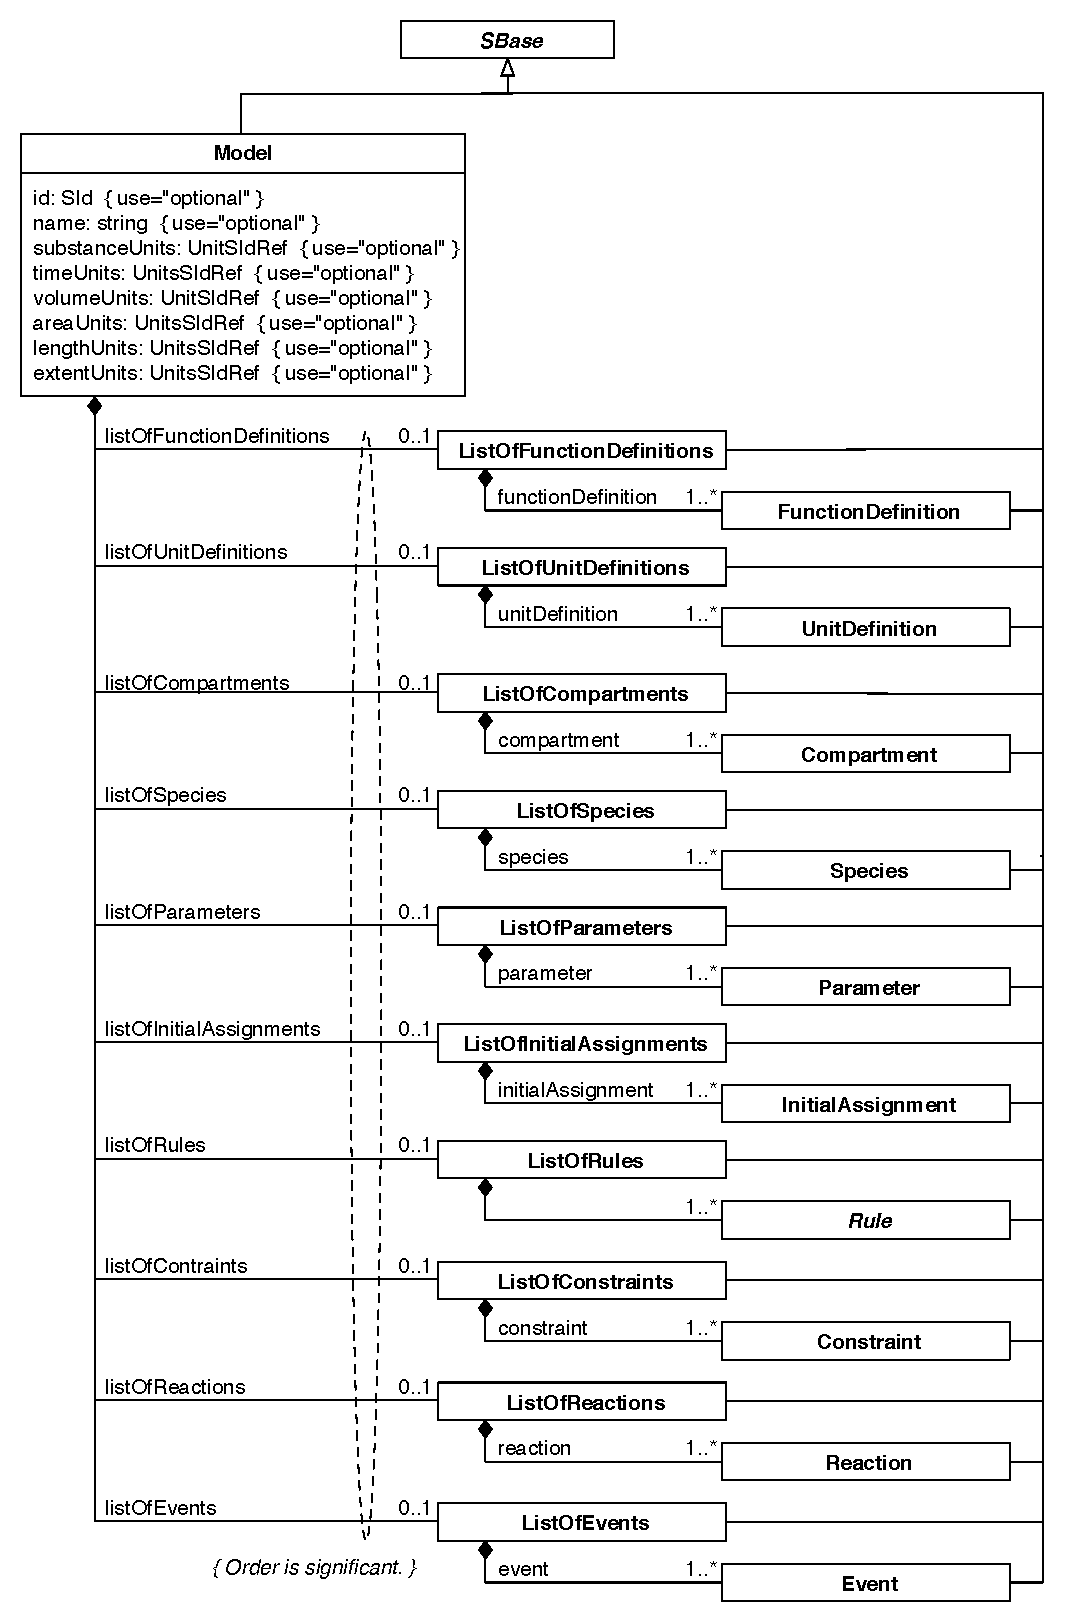
\includegraphics[scale=0.76]{figs/model-uml}
  \caption{The definition of \Model and the many helper
      classes \ListOfFunctionDefinitions, \ListOfUnitDefinitions,
      \ListOfCompartments, \ListOfSpecies, \ListOfParameters,
      \ListOfInitialAssignments, \ListOfRules, \ListOfConstraints,
      \ListOfReactions, and \ListOfEvents.}
  \label{fig:model}
\end{figure}

The \Model object has an optional attribute, \token{id}, used to
give the model an identifier.  The identifier must be a text
string conforming to the syntax permitted by the \primtype{SId}
data type described in Section~\ref{sec:sid}.  \Model also has an
optional \token{name} attribute, of type \primtype{string}.  The
\token{name} and \token{id} attributes must be used as described in
Section~\ref{sec:idnameattribs}.

\Model serves as a container for components of classes
\FunctionDefinition, \UnitDefinition, \Compartment, \Species, \Parameter,
\InitialAssignment, \Rule, \Constraint, \Reaction and \Event.
Instances of the classes are placed inside instances of classes
\ListOfFunctionDefinitions, \ListOfUnitDefinitions,
\ListOfCompartments, \ListOfSpecies, \ListOfParameters, \ListOfInitialAssignments,
\ListOfRules, \ListOfConstraints, \ListOfReactions, and
\ListOfEvents.  The ``list'' classes are defined in
Figure~\ref{fig:model}.  All of the lists are optional, but if a
given list container is present within the model, the list must
not be empty; that is, it must have length one or more.  The
resulting XML data object for a full model containing every
possible list would have the following form:

\newcommand{\sayOptional}{\raisebox{0pt}[0pt][0pt]{\bigg\} \textrm{\emph{optional}}}}

\vspace*{1.5ex}
\begin{tt}
  \tightspacing
  \small
  \begin{tabbing}
xxxx\=xxxx\=xxxx\=xxxx\=xxxx\=\kill
\+\>
<?xml version="1.0" encoding="UTF-8"?>\\
<sbml xmlns="http://www.sbml.org/sbml/level3/version1/core" level="3" version="1">\\
\><model id="My\_Model">\\
\>\><listOfFunctionDefinitions>\\
\>\>\>\textrm{\emph{one or more}} <functionDefinition> ... </functionDefinition> \textrm{\emph{elements}}  \` \sayOptional\\
\>\></listOfFunctionDefinitions>\\
\>\><listOfUnitDefinitions>\\
\>\>\>\textrm{\emph{one or more}} <unitDefinition> ... </unitDefinition> \textrm{\emph{elements}}  \` \sayOptional\\
\>\></listOfUnitDefinitions>\\
\>\><listOfCompartments>\\
\>\>\>\textrm{\emph{one or more}} <compartment> ... </compartment> \textrm{\emph{elements}}  \` \sayOptional\\
\>\></listOfCompartments>\\
\>\><listOfSpecies>\\
\>\>\>\textrm{\emph{one or more}} <species> ... </species> \textrm{\emph{elements}}  \` \sayOptional\\
\>\></listOfSpecies>\\
\>\><listOfParameters>\\
\>\>\>\textrm{\emph{one or more}} <parameter> ... </parameter> \textrm{\emph{elements}}  \` \sayOptional\\
\>\></listOfParameters>\\
\>\><listOfInitialAssignments>\\
\>\>\>\textrm{\emph{one or more}} <initialAssignment> ... </initialAssignment> \textrm{\emph{elements}}  \` \sayOptional\\
\>\></listOfInitialAssignments>\\
\>\><listOfRules>\\
\>\>\>\textrm{\emph{one or more elements of subclasses of \abstractclass{Rule}}}  \` \sayOptional\\
\>\></listOfRules>\\
\>\><listOfConstraints>\\
\>\>\>\textrm{\emph{one or more}} <constraint> ... </constraint> \textrm{\emph{elements}}  \` \sayOptional\\
\>\></listOfConstraints>\\
\>\><listOfReactions>\\
\>\>\>\textrm{\emph{one or more}} <reaction> ... </reaction> \textrm{\emph{elements}}  \` \sayOptional\\
\>\></listOfReactions>\\
\>\><listOfEvents>\\
\>\>\>\textrm{\emph{one or more}} <event> ... </event> \textrm{\emph{elements}}  \` \sayOptional\\
\>\></listOfEvents>\\
\></model>\\
</sbml>
\end{tabbing}
\regularspacing
\end{tt}
\vspace*{1ex}

Although all the lists are optional, there are dependencies
between SBML components such that defining some components
requires defining others.  An example is that defining a species
requires defining a compartment, and defining a reaction requires
defining a species.  The dependencies are explained throughout the
text.
  

\subsubsection{The \token{sboTerm} attribute}
\label{sec:model-sboterm}

\Model inherits an optional \token{sboTerm}
attribute of type \primtype{SBOTerm} from its parent
class \SBase (see Sections~\ref{sec:sboterm-type}
and~\ref{sec:sboTerm}).  When a value is given to this
attribute in a \Model instance, it should be an
SBO identifier belonging to the branch for type \Model 
indicated in Table~\ref{tab:sboterm-availability}. 
The term chosen should be the most precise (narrow)
one that captures the overall process or phenomenon represented
by the overall SBML model.

As discussed in Section~\ref{sec:sboTerm}, SBO labels are optional
information on a model.  Applications are free to ignore
\token{sboTerm} values.  A model must be interpretable without the
benefit of SBO labels.

\subsubsection{The \token{substanceUnits} attribute}
\label{sec:model-substanceUnits}

This attribute specifies the units in which the substance of a
\Species is measured within the model. The value must be of type
\primtype{UnitSIdRef} (Section:~\vref{sec:unitsidref}). This value
can be changed for individual species
(Section:~\vref{sec:species}). A list of recommended units is
given in section~\vref{sec:bp:unitdefinitions:recommendedunits:substanceUnits}. 

\subsubsection{The \token{timeUnits} attribute}
\label{sec:model-timeUnits}

This attribute specifies the units in which the time is measured
within the model. The value must be of type \primtype{UnitSIdRef}
(Section:~\vref{sec:unitsidref}). A list of recommended units is given in
section~\vref{sec:bp:unitdefinitions:recommendedunits:timeUnits}. 

\subsubsection{The \token{volumeUnits} attribute}
\label{sec:model-volumeUnits}

This attribute specifies the units in which the volume of a
\Compartment of \token{spatialDimensions} 3 is measured within the model. The
value must be of type \primtype{UnitSIdRef}
(Section:~\vref{sec:unitsidref}). This value can be changed for
individual compartments (Section:~\vref{sec:compartments}). A
list of recommended units is given in
section~\vref{sec:bp:unitdefinitions:recommendedunits:volumeUnits}.  

\subsubsection{The \token{areaUnits} attribute}
\label{sec:model-areaUnits}

This attribute specifies the units in which the area of a
\Compartment of \token{spatialDimensions} 2 is measured within the model. The
value must be of type \primtype{UnitSIdRef}
(Section:~\vref{sec:unitsidref}). This value can be changed for
individual compartments (Section:~\vref{sec:compartments}). A
list of recommended units is given in
section~\vref{sec:bp:unitdefinitions:recommendedunits:areaUnits}.  

\subsubsection{The \token{lengthUnits} attribute}
\label{sec:model-lengthUnits}

This attribute specifies the units in which the length of a
\Compartment of \token{spatialDimensions} 1 is measured within the model. The
value must be of type \primtype{UnitSIdRef}
(Section:~\vref{sec:unitsidref}). This value can be changed for
individual compartments (Section:~\vref{sec:compartments}). A
list of recommended units is given in
section~\vref{sec:bp:unitdefinitions:recommendedunits:lengthUnits}.  

\subsubsection{The \token{extentUnits} attribute}
\label{sec:model-extentUnits}

This attribute specifies the units in which the extent of
{\Reaction}s is measured within the model. The value must be of
type \primtype{UnitSIdRef} (Section:~\vref{sec:unitsidref}). A
list of recommended units is given in 
section~\vref{sec:bp:unitdefinitions:recommendedunits:extentUnits}. 

\subsubsection{The \token{conversionFactor} attribute}
\label{sec:model-conversionFactor}
\todo{sven}{Write me.}


\subsubsection{The ListOf container classes}
\label{sec:listof}
\label{sec:listofunitdefinitions}
\label{sec:listoffunctiondefinitions}
\label{sec:listofcompartments}
\label{sec:listofspecies}
\label{sec:listofparameters}
\label{sec:listofinitialassignments}
\label{sec:listofinitialassign}
\label{sec:listofrules}
\label{sec:listofconstraints}
\label{sec:listofreactions}
\label{sec:listofevents}

The various \ListOf classes defined in Figure~\ref{fig:model}
are merely containers used for organizing the main components of
an SBML document.  All are derived from the abstract class \SBase
(Section~\ref{sec:sbase}), and inherit \SBase's various attributes
and subelements such as \token{metaid} and \token{annotation},
although in SBML \thisLVR there are no defined SBO terms for the
\token{sboTerm} attribute.  The \ListOf classes do not add any
attributes of their own.

There are several motivations for grouping SBML components within XML elements named after \token{listOfClassNames}, rather than
placing the components all directly at the top level.  First, the
fact that the container classes are derived from \SBase means that
software tools can add information about the lists themselves into
each list container's \token{annotation}, a feature that a number
of today's software tools exploit.  Second, we believe the
grouping leads to a more modular structure that is helpful when
working with elements from multiple SBML Level~3 packages.  Third,
we believe that it makes visual reading of models in XML easier,
for situations when humans must inspect and edit SBML directly.

%Prior to \sbmltwofour, the SBML specifications stipulated that the
%SBO branch for \Model had be the mathematical framework
%branch of SBO.  This turned out to be confusing and problematic.
%A realization also occurred in the SBML community that a
%model is, ultimately, always a representation of some 
%process or phenomenon involving different entities, making the SBO
%branch of \sbointeraction, an appropriate one for the
%\token{sboTerm} value on an SBML \Model.



%-----------------------------------------------------------------------------
\subsection{Function definitions}
\label{sec:functiondefinition}
%-----------------------------------------------------------------------------

The \FunctionDefinition object associates an identifier with a
function definition.  This identifier can then be used as the
function called in subsequent MathML \token{apply} elements.
\FunctionDefinition is shown in Figure~\ref{fig:mathdefinition}.

\begin{figure}[htb]
  \centering
  \small
  \begin{tikzpicture}
    \node[above=0.4in] (a) {
      \emptyClassbox{\textsl{SBase}}
    };
    \node (b) {
      \begin{classbox}{\textcolor{black}{FunctionDefinition}}
        id: SId                           \\
        name: string \{ use="optional" \} \\
      \end{classbox}
    };
    \node[right=1.6in] (c) {
      \begin{classbox}{Lambda}
        xmlns: string \{ "http://www.w3.org/1998/Math/MathML" \} \\
        \{ \emph{\mathml content restricted to one \mathml \token{lambda}} \\[-1pt]
        \emph{or one \token{semantics} element containing a \token{lambda}. \}} \\
      \end{classbox}
    };
    \draw[open triangle 60-] (a) -- (b);
    \draw[diamond-,shorten <=-7pt,shorten >=-6pt] (b) -- (c)
        node[above=6pt,left=1.8in] {\textsf{math}};
  \end{tikzpicture}
  \caption{The definition of class \FunctionDefinition.
      The contents of the \class{Lambda} class is a single \mathml
      \token{lambda} expression (or a \token{lambda} surrounded by
      a \token{semantics} element).  A function definition must
      contain exactly one \token{math} element defined by the
      \class{Lambda} class; note also that \class{Lambda} is not
      derived from \SBase, which means that the attributes defined
      on \SBase are \emph{not} available on the \token{math}
      element.  A sequence of one or more instances of
      \FunctionDefinition objects can be located in an instance of
      \ListOfFunctionDefinitions in \Model, as shown in
      Figure~\protect\ref{fig:model}.}
  \label{fig:mathdefinition}
  \label{fig:functionDefinition}
\end{figure}

Function definitions in SBML (also informally known as
``user-defined functions'') have purposefully limited capabilities.
As is made more clear below, a function cannot reference
parameters or other model quantities outside of itself; values
must be passed as parameters to the function.  Moreover, recursive
and mutually-recursive functions are not permitted.  The purpose
of these limitations is to balance power against complexity of
implementation.  With the restrictions as they are, function
definitions could be implemented as textual substitutions---they
are simply macros.  Software implementations therefore do not need
the full function-definition machinery typically associated with
programming languages.


\subsubsection{The \token{id} and \token{name} attributes}

The \token{id} and \token{name} attributes have types \primtype{SId}
and \primtype{string}, respectively, and operate in the manner
described in Section~\ref{sec:idnameattribs}.  MathML \token{ci}
elements in an SBML model can refer to the function defined by a
\FunctionDefinition using the value of its \token{id} attribute.


\subsubsection{The \token{math} element}
\label{sec:function-definition-math}



The \token{math} element is a container for MathML
content that defines the function.  The content of this
element can only be a MathML \token{lambda} element
or a MathML \token{semantics} element containing a
  \token{lambda} element.  The \token{lambda} element must begin
with zero or more \token{bvar} elements, followed by any other of
the elements in the MathML subset listed in
Section~\ref{sec:mathmlsubset} \emph{except} \token{lambda} (\ie a
\token{lambda} element cannot contain another \token{lambda}
element).  This is the only place in SBML where a \token{lambda}
element can be used.



A further restriction on the content of \token{math} is that it
cannot contain references to variables other than the variables
declared to the \token{lambda} itself.  That is, the contents of
MathML \token{ci} elements inside the body of the \token{lambda}
can only be the variables declared by its \token{bvar} elements,
or the identifiers of other \FunctionDefinition{}s defined in
the same model.  This restriction also applies to the
  \token{csymbol} for \quantity{time}.  Functions must be written
so that all variables or parameters used in the MathML content are
passed to them via their function parameters.


\subsubsection{The \token{sboTerm} attribute}
\label{sec:functiondefinition-sboterm}

\FunctionDefinition inherits an optional \token{sboTerm}
attribute of type \primtype{SBOTerm} from its parent
class \SBase (see Sections~\ref{sec:sboterm-type}
and~\ref{sec:sboTerm}).  When a value is given to this
attribute in a \FunctionDefinition instance, it should be an
SBO identifier belonging to the branch for type \FunctionDefinition 
indicated in Table~\ref{tab:sboterm-availability}.  The relationship is
of the form ``the function definition \emph{is a} X'', where X is
the SBO term.  The term chosen should be the most precise (narrow)
one that captures the role of the function in the model.

As discussed in Section~\ref{sec:sboTerm}, SBO labels are optional
information on a model.  Applications are free to ignore
\token{sboTerm} values.  A model must be interpretable without the
benefit of SBO labels.




\subsubsection{Calling user-defined functions}
\label{sec:functiondefinition-calling}

Within MathML expressions in an SBML model, all calls to a
function defined by a \FunctionDefinition must use the same number
of arguments as specified in the function's definition.  The
number of arguments is equal to the number of \token{bvar}
elements inside the \token{lambda} element of the function
definition.



Note that \FunctionDefinition does not have a separate attribute
for defining the units of the value returned by the function.  The
units associated with the function's return value, when the
function is called from within MathML expressions elsewhere in
SBML, are simply the overall units of the expression in \FunctionDefinition's
\token{math} when applied to the arguments supplied in the call to
the function.  Ascertaining these units requires performing
dimensional analysis on the expression.  (Readers may wonder why
there is no attribute.  The reason is that having a separate
attribute for declaring the units would not only be redundant, but
also lead to the potential for having conflicting information.  In
the case of a conflict between the declared units and those of the
value actually returned by the function, the only logical
resolution rule would be to assume that the correct units are
those of the expression anyway.)


\subsubsection{Examples}

The following abbreviated SBML example shows a \FunctionDefinition
object instance defining \token{pow3} as the identifier of a function
computing the mathematical expression $x^{3}$, and after that, the
invocation of that function in the mathematical formula of a rate
law.  Note how the invocation of the function uses its identifier.

\begin{example}
<model>
    ...
    <listOfFunctionDefinitions>
        <functionDefinition id="pow3">
            <math xmlns="http://www.w3.org/1998/Math/MathML">
                <lambda>
                    <bvar><ci> x </ci></bvar>
                    <apply>
                        <power/>
                        <ci> x </ci>
                        <cn> 3 </cn>
                    </apply>
                </lambda>
            </math>
        </functionDefinition>
    </listOfFunctionDefinitions>
    ...
    <listOfReactions>
        <reaction id="reaction_1" reversible="true" fast="false">
            ...
            <kineticLaw>
                <math xmlns="http://www.w3.org/1998/Math/MathML">
                    <apply>
                        <ci> pow3 </ci>
                        <ci> S1 </ci>
                     </apply>
                </math>
            </kineticLaw>
            ...
        </reaction>
    </listOfReactions>
    ...
</model>\end{example}


%-----------------------------------------------------------------------------
\subsection{Unit definitions}
\label{sec:unitdefinitions}
%-----------------------------------------------------------------------------

Units of measurement may be supplied in a number of contexts in an
SBML model.  The units of the following mathematical entities can
be specified explicitly: the time of the \Model, the size of a
\Compartment, the amount/substance of a \Species, the units of
constant and variable \Parameter values, and the units of the 
extent of a \Reaction.  The overall units of any mathematical
formula appearing in SBML are those that arise naturally from the
components and mathematical expressions comprising the formula, or
in other words, the units obtained by doing dimensional analysis
on the formula.

Rather than requiring a complete unit definition on every object,
SBML provides a facility for defining units that can be referenced
throughout a model.  The SBML unit definition facility uses two
classes of objects, \UnitDefinition and \Unit.  Their definitions
are shown in Figure~\vref{fig:unitdefinition} and explained in
more detail in Sections~\ref{sec:unitdefinition-structure}
and~\ref{sec:unit-structure} below.

\begin{figure}[htb]
  \centering
  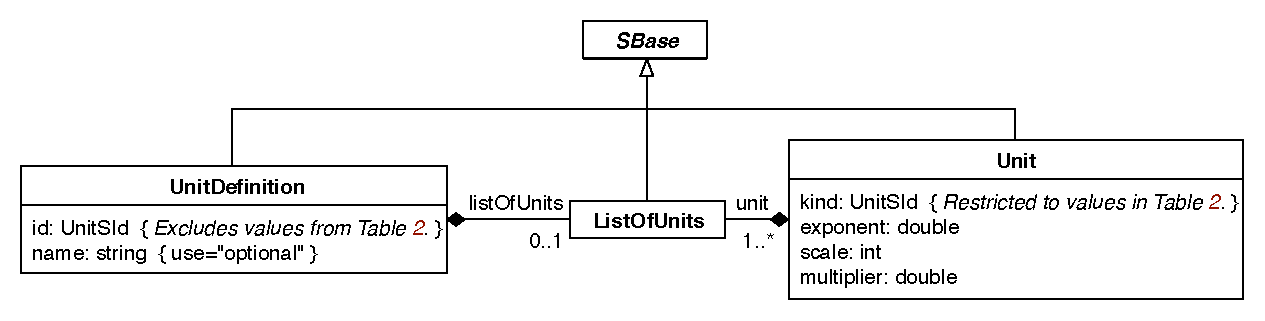
\includegraphics[scale=0.79]{figs/unitdefinition-uml}
  \caption{The definition of classes \UnitDefinition and
      \Unit.  A sequence of one or more instances of
      \UnitDefinition can be located in an instance of
      \ListOfUnitDefinitions in \Model
      (Figure~\protect\ref{fig:model}).  \class{ListOfUnits} has
      no attributes (beyond those it inherits from class \SBase);
      it merely acts as a container for one or more instances of
      \Unit objects.  Note that the only permitted values of
      \token{kind} on \Unit are the reserved words in
      Table~\vref{tab:unitkind}, but these symbols are
      \emph{excluded} from the permitted values of
      \UnitDefinition's \token{id} because SBML's unit system does
      not allow redefining the base units.}
  \label{fig:unitdefinition}
\end{figure}

The approach to defining units in SBML is compositional; for
example, $meter\ second^{\,-2}$ is constructed by combining a
\Unit object representing $meter$ with another \Unit object
representing $second^{\,-2}$.  The combination is wrapped inside a
\UnitDefinition, which provides for assigning an identifier and
optional name to the combination.  The identifier can then be
referenced from elsewhere in a model.

The vast majority of modeling situations requiring new SBML unit
definitions involve simple multiplicative combinations of base
units and factors.  An example of this might be ``moles per litre
per second''.  What distinguishes these sorts of simpler unit
definitions from more complex ones is that they may be expressed
without the use of an additive offset from a zero point.  The use
of offsets complicates all unit definition systems, yet in the
domain of SBML the real-life cases requiring offsets are few (and
in fact, to the best of our knowledge, only involve temperature).
Consequently, the SBML unit system has been consciously designed
in a way that attempts to simplify implementation of unit support
for the most common cases in systems biology, at the cost of
requiring units with offsets to be handled explicitly by the
modeler.


\subsubsection{\class{UnitDefinition}}
\label{sec:unitdefinition-structure}

A unit definition in SBML consists of an instance of a
\UnitDefinition object, shown in Figure~\ref{fig:unitdefinition}.


\paragraph{The \token{id} and \token{name} attributes}

The required attribute \token{id} and optional attribute
\token{name} have data types \primtype{UnitSIdRef} (Section
\ref{sec:unitsidref}) and \primtype{string}, respectively.  The
\token{id} attribute is used to give the defined unit a unique
identifier by which other parts of an SBML model definition can
refer to it.  The \token{name} attribute is intended to be used
for giving the unit definition an optional human-readable name;
see Section~\ref{sec:name} for more guidelines about the use of
names.

There is one important restrictions about the use of unit
definition \token{id} values: 
\begin{enumerate}
  
\item The \token{id} of a \UnitDefinition must \emph{not} contain
  a value from Table~\ref{tab:unitkind}, the list of
  reserved base unit names.  This constraint simply prevents
  the redefinition of base units.

\end{enumerate}


\paragraph{The list of \class{Unit}s}
\label{sec:listofunits}

A \UnitDefinition object may contain a \ListOfUnits container which must
contain one or more \Unit objects. Section~\ref{sec:unit-structure} explains
the meaning and use of \Unit.   

\paragraph{Example}

The following skeleton of a unit definition illustrates an example
use of \UnitDefinition:

\begin{example}

<model>
    <listOfUnitDefinitions>
        <unitDefinition id="unit1">
            <listOfUnits>
                ...
            </listOfUnits>
        </unitDefinition>
        <unitDefinition id="unit2">
            <listOfUnits>
                ...
            </listOfUnits>
        </unitDefinition>
    </listOfUnitDefinitions>
    ...
</model>
\end{example}


\subsubsection{\class{Unit}}
\label{sec:unit-structure}

A \Unit object represents a (possibly transformed) reference to
a base unit chosen from the list in
  Table~\vref{tab:unitkind}.  The attribute
\token{kind} indicates the chosen base unit, whereas the
attributes \token{exponent}, \token{scale}, and
\token{multiplier} define how the base unit is being transformed.
These various attributes are described in detail below.


\paragraph{The \token{kind} attribute}

% Aliases for bibliography entries, to compensate for some labeling issues.

\defcitealias{bipm:1998}{BIPM, 1998}
\defcitealias{bipm:2000}{BIPM, 2000}

The \Unit object class has four required attributes, the first being
\token{kind}, whose value must be taken from the list of reserved
words given in Table~\vref{tab:unitkind}.  These reserved
symbols are defined in the value space of \primtype{UnitSId}
(Section \ref{sec:unitsid}).

\begin{table}[bht]
  \centering
  \ttfamily
  \small
  \vspace*{-0.5ex}
  \setlength{\arraycolsep}{8pt}
  \begin{edtable}{tabular}{@{}llllll@{}}
    \toprule
    ampere    & farad   & joule    & lux    & radian    & volt\\
    \underline{avogadro} & gram    & katal  & metre     & second  & watt \\
    becquerel & gray    & kelvin   & mole   & siemens   & weber\\
    candela   & henry   & kilogram & newton & sievert   \\
    coulomb   & hertz   & litre    & ohm    & steradian \\
    \underline{dimensionless} & \underline{item} & lumen & pascal & tesla\\
     farad    & joule   & lux      & radian    & volt   \\
    \bottomrule
  \end{edtable}
  \vspace*{-0.5ex}
  \caption{Base units defined in SBML.  These symbols are
    predefined values of type \primtype{UnitSId}
    (Section~\ref{sec:unitsid}).  All are names of base or derived
    SI units~\protect\citep{bipm:2006}, except for
    ``\token{avogadro}'', ``\token{dimensionless}'' and
    ``\token{item}'', which are SBML additions important for
    handling certain common situations.  ``\token{Dimensionless}''
    is intended for cases where a quantity is a ratio whose units
    cancel out, the unit ``\token{avogadro}'' is the unit
    ``\token{Dimensionless}'' multiplied with Avogadro's number,
    and ``\token{item}'' is used for expressing such things as 
    ``N items'' (e.g., ``100 molecules'').  Also, note that the
    gram and litre are not strictly part of SI; however, they are
    frequently used in SBML's areas of application and therefore
    are included as predefined unit identifiers.  (The standard SI
    unit of mass is in fact the kilogram, and volume is defined in
    terms of cubic metres.)  Comparisons of these values, like all
    values of type \primtype{UnitSId}, must performed in a
    case-sensitive manner.}
  \label{tab:unitkind}
\end{table}

Note that the set of acceptable values for the attribute \token{kind}
does \emph{not} include units defined by \UnitDefinition
object.  This means that the units definition system
in SBML is not hierarchical: user-defined units cannot be built on
top of other user-defined units, only on top of base units.


\paragraph{The \token{exponent} attribute}
\label{sec:unit-structure:exponent}

The \token{exponent} attribute on \Unit specifies an exponent on
the base unit given by the \token{kind} attribute. This allows the
definition of a new unit cubic meter which can be defined as the base
unit metre with an exponent 3. 

\paragraph{The \token{scale} attribute}
\label{sec:unit-structure:scale}

A \Unit object also has a \token{scale} attribute; its
value must be an integer exponent for a power-of-ten multiplier
used to set the scale of the unit.  For example, a unit having a
\token{kind} value of \val{gram} and a \token{scale} value of
\val{-3} signifies $10^{-3} \times gram$, or milligrams.  To avoid
scaling the value of \token{scale} must be set to \val{0} (zero),
because $10^0 = 1$.  

\paragraph{The \token{multiplier} attribute}
\label{sec:unit-structure:multiplier}

The \token{multiplier} attribute can be used to multiply the
\token{kind} unit by a real-numbered factor; this enables the
definition of units that are not power-of-ten multiples of SI
units.  For instance, a \token{multiplier} of 0.3048 could be used
to define \val{foot} as a measure of length in terms of a metre. 

\paragraph{Sematics of \Unit}
\label{sec:unit-structure:semantics}

\newcommand{\ynew}{\ensuremath{y}\xspace}
\newcommand{\ybase}{\ensuremath{y_b}\xspace}
\newcommand{\unew}{\ensuremath{\{u\}}\xspace}
\newcommand{\ubase}{\ensuremath{\{u_b\}}\xspace}
\newcommand{\uone}{\ensuremath{\{u_{b_1}\}}\xspace}
\newcommand{\utwo}{\ensuremath{\{u_{b_2}\}}\xspace}
\newcommand{\un}  {\ensuremath{\{u_{b_n}\}}\xspace}

The unit \unew given by the \Unit element is defined as:
\begin{linenomath}
\begin{equation}
  \unew = (\token{multiplier} \cdot 10^\token{scale} \, \ubase)^\token{exponent}
\label{eq:unit-semantics}
\end{equation}
\end{linenomath}
Here \ubase denotes the base unit specified by the \token{kind}
attribute. 

The new unit \unew given by an \UnitDefinition is defined as the
product all \Unit elements contained in the \ListOfUnits: 
\begin{linenomath}
\begin{equation}
  \unew = \{u_1\} \, \{u_2\} \, \ldots \, \{u_n\} 
\label{eq:unitDefinition-semantics}
\end{equation}
\end{linenomath}
Let the value of the \token{multiplier} of unit $\{u_i\}$ be
$m_i$. Similarly let the value of the \token{scale} be $s_i$ and the value
of the \token{exponent} be $x_i$. We can then write the above as:
\begin{linenomath}
\begin{align}
  \{u\} &= (m_1 \cdot 10^{s_1} \uone)^{x_1} \cdot
           (m_2 \cdot 10^{s_2} \utwo)^{x_2} \cdot \ldots \cdot (m_n \cdot
           10^{s_n} \un)^{x_n} \notag \\[2pt]
        &= m_1^{x_1} \cdot m_2^{x_2} \cdot \ldots \cdot m_n^{x_n}
           \cdot 10^{(s_1 x_1 + s_2 x_2 + \ldots + s_n x_n)}
           \cdot \uone^{x_1} \utwo^{x_2} \ldots \un^{x_n} \notag \\[2pt]
        &= m \cdot 10^{s} \cdot \uone^{x_1} \utwo^{x_2} \ldots \un^{x_n}
\label{eq:multip-units}
\end{align}
\end{linenomath}
where we used:
\begin{linenomath}
\begin{align}
  m &= m_1^{x_1} \cdot m_2^{x_2} \cdot \ldots \cdot m_n^{x_n} \notag\\
  s &= s_1 x_1 + s_2 x_2 + \ldots + s_n x_n \notag\\
\end{align}
\end{linenomath}

\paragraph{Examples}

The following example illustrates the definition of an
abbreviation \val{mmls} for the units $mmol\ l^{-1}\ s^{-1}$:

\begin{example}
<listOfUnitDefinitions>
    <unitDefinition id="mmls">
        <listOfUnits>
            <unit kind="mole"   exponent="1"  scale="-3" multiplier="1"/>
            <unit kind="litre"  exponent="-1" scale="0"  multiplier="1"/>
            <unit kind="second" exponent="-1" scale="0"  multiplier="1"/>
        </listOfUnits>
    </unitDefinition>
</listOfUnitDefinitions>
\end{example}

\paragraph{Comparing Units}
The unit system allows model quantities to be expressed in units
other than the base units of Table~\ref{tab:unitkind}.  For
analyses and computations, the consumer of the model (be it a
software tool or a human) will want to convert all model
quantities to base SI units for purposes such as verifying the
consistency of units throughout the model. Let us look at a
quantity measuered in base units and a defined unit \unew. The
value of the quantity will be \ybase in the base units and \ynew
in \unew. Since the quantity does not change we have the following
equality:

\begin{linenomath}
\begin{equation}
  \ybase \, \uone^{z_1} \utwo^{z_2} \ldots \un^{z_n}
     = \ynew \, \unew 
\label{eq:unit-equality}
\end{equation}
\end{linenomath}
where the unkown exponents of the base units are denoted with
$z_i$. Substituting \unew in Equation~\ref{eq:unit-equality} with
Equation~\ref{eq:multip-units} we obtain.
\begin{linenomath}
\begin{equation}
  \ybase \, \uone^{z_1} \utwo^{z_2} \ldots \un^{z_n}
    = \ynew \cdot m \cdot 10^s \, \uone^{x_1} \utwo^{x_2} \ldots \un^{x_n}
\label{eq:unit-conversion}
\end{equation}
\end{linenomath}
Using the independence of the base units we can derive the unkown
exponents $z_i = x_i$ and that $\ybase = \ynew \cdot m \cdot 10^s$.

Please note that when comparing units that in addition to the relationships defined by the SI Units~\protect\citep{bipm:2006} the following special relationship must be considered: 
\begin{linenomath}
\begin{equation}
  \mbox{mole} = \mbox{avogadro} * \mbox{item}
\label{eq:unit-conversion-avogadro}
\end{equation}
\end{linenomath}

\label{sec:unit-simple-approach}
Some additional points are worth discussing about the unit scheme
introduced so far.  First, and most importantly, the equations
above are formulated with the assumption that the base units do
not require an additive offset as part of their definition.
\emph{When temperature values in units other than kelvin are being
  considered, then a different interpretation must be made}, as
discussed below.

A second point is that care is needed to avoid seemingly-obvious
but incorrect translations of units described in textbooks.  The
scheme above makes it easy to formulate statements such as ``1
foot = 0.3048 metres'' in the most natural way.  However, the most
common expression of the relationship between temperature in
Fahrenheit and kelvin, ``$T_{Fahrenheit} = 1.8 \cdot (T_{kelvin} -
273.15) + 32$'' might lead one to believe that defining Fahrenheit
degrees in terms of kelvin degrees involves using
\token{multiplier}=\val{1.8}.  \emph{Not so}, when degree changes
are being considered and not temperature values.  Converting
\emph{temperature values} is different from expressing a
relationship between degree measurements.  The proper value for
the multiplier in the latter case is $5/9$, \ie
\token{multiplier}=\val{0.555556} (where we picked an arbitrary
decimal precision).  If, on the other hand, the actual temperature
is relevant to a quantity (\eg if a model uses a quantity that has
particular values at particular temperatures), then offsets are
required in the unit calculations and a formula must be used as
discussed above.

While SBML no longer allows to directly specify offsets  on units, it is still possible
to encode models using such units. For more information on \emph{how to best 
handle units requiring the use of offsets} see \ref{sec:bp:unitdefinitions:offset}. 

\subsubsection{References to units}

An attribute that defines the units of a mathematical entity (\eg the
attribute \token{units} on \Parameter) can refer to a defined unit
whose identifier is chosen from among the following:
\begin{itemize}
  
\item A new unit identifier defined by a \UnitDefinition as
  described at the start of Section~\ref{sec:unitdefinitions};

\item The base units listed in Table~\vref{tab:unitkind}; and
  
\end{itemize}

Software developers are asked to pay special attention to the
units used in an SBML model.  Different users and developers
sometimes are accustomed to making different assumptions about
units, and these assumptions may not correspond to what is
actually defined in SBML.  The numerical values in a model become
meaningless if the corresponding units are not those being
assumed.  Sections~\ref{sec:ci-token}, \ref{sec:species-units} and
\ref{subsec:kinetic-law} have particularly important notes about
the usage of units in SBML.

%-----------------------------------------------------------------------------
\subsection{Compartments}
\label{sec:compartments}
%-----------------------------------------------------------------------------

A \emph{compartment} in SBML represents a bounded space in which
species are located.  Compartments do not necessarily have to
correspond to actual structures inside or outside of a biological
cell, although models are often designed that way.  The definition
of \Compartment is shown in Figure~\vref{fig:compartment}.

\begin{figure}[htb]
  \centering
  \small
  \vspace*{-1ex}
  \begin{tikzpicture}
    \node[above=0.9in] (a) {
      \emptyClassbox{\textsl{SBase}}
    };
    \node (b) {
      \begin{classbox}{Compartment}
        id: SId \\
        name: string \{ use="optional" \} \\
        spatialDimensions: double \{ use="optional" \} \\
        size: double \{ use="optional" \} \\
        units: UnitSIdRef \{ use="optional" \} \\
        constant: boolean \\
      \end{classbox}
    };
    \draw[open triangle 60-] (a) -- (b);
  \end{tikzpicture}
  \caption{The definition of class \Compartment.  A
      sequence of one or more instances of \Compartment objects
      can be located in an instance of \ListOfCompartments in
      \Model, as shown in Figure~\protect\ref{fig:model}.}
  \label{fig:compartment}
\end{figure}

It is important to note that although compartments are optional in
the overall definition of \Model (see Section~\ref{sec:model}),
every species in an SBML model must be located in a compartment.
This in turn means that if a model defines any species, the model
must also define at least one compartment.  The reason is simply
that species represent physical things, and therefore must exist
\emph{somewhere}.  Compartments represent the \emph{somewhere}.


\subsubsection{The \token{id} and \token{name} attributes}

\Compartment has one required attribute, \token{id}, of type
\primtype{SId}, to give the compartment a unique identifier by
which other parts of an SBML model definition can refer to it.  A
compartment can also have an optional \token{name} attribute of type
\primtype{string}.  Identifiers and names must be used according
to the guidelines described in Section~\ref{sec:idnameattribs}.



\subsubsection{The \token{spatialDimensions} attribute}

A \Compartment object has an optional floating-point attribute named
\token{spatialDimensions}, indicating the spatial dimensions possessed by the
compartment. Note that the \token{spatialDimensions} attribute is more akin to an 
annotation in that its value cannot alter the mathematics of the model. 

\subsubsection{The \token{size} attribute}
\label{sec:size}

Each compartment has an optional floating-point attribute named
\token{size}, representing the initial total size of the
compartment.  The size may be a volume (if the compartment is a
three-dimensional one), or it may be an area (if the compartment
is two-dimensional), or a length (if the compartment is
one-dimensional).

It is important to note that in SBML Level~3, a missing
\token{size} value \emph{does not imply that the compartment size
  is 1}. A missing value for \token{size} for a given
compartment signifies that the value either is unknown, or to be
obtained from an external source, or determined by an initial
assignment (Section~\ref{sec:initialAssignment}) or a rule
(Section~\ref{sec:rules}) elsewhere in the model.  \

A compartment's size is set by its \token{size}
attribute exactly once.  If the compartment's
\token{constant} attribute value is \val{true}, then the size is 
fixed and cannot be changed except by
an \InitialAssignment in the model.  These methods of setting the size
differ in that the \token{size} attribute can only be used to set
the compartment size to a literal scalar value, whereas
\InitialAssignment allows the value to be set using an arbitrary
mathematical expression.  If the compartment's \token{constant}
attribute is \val{false}, the size value may be overridden by an
\InitialAssignment or changed by an \AssignmentRule or
\AlgebraicRule, and in addition, for simulation time $t > 0$, it
may also be changed by a \RateRule or \Event{}s.  (However, some
constructs are mutually exclusive; see Sections~\ref{sec:rules}
and~\ref{sec:events}.)  It is not an error to set the value of \token{size}
on a compartment and also redefine the value using an
\InitialAssignment, but the original \token{size} value in that case is
ignored.  Section~\ref{sec:before-t0} provides additional
information about the semantics of assignments, rules and values
for simulation time $t \leq 0$.

For the reasons given above, the \token{size} attribute on a
compartment must be defined as optional; however, \emph{it is
  extremely good practice to specify values for compartment sizes}
when such values are available. The reasons for this are explained
in Section~\ref{sec:bp:size}.


\subsubsection{The \token{units} attribute}
\label{sec:compartment-units}

The units associated with the compartment's \token{size} value may
be set using the optional attribute \token{units}.  The value must
be of type \primtype{UnitSIdRef}
(Section:~\vref{sec:unitsidref}). In the case that the attribute
\token{units} is not given the units may be inherited from the
model as specified in Table~\ref{tab:comp-size-units}. A list of
recommended units is given in
section~\vref{sec:bp:unitdefinitions:recommendedunits:sizeUnits}. 
  
\begin{table}[h]
  \small
  \centering
  \vspace*{-1ex}
  \begin{edtable}{tabular}{cl}
    \toprule
    \textbf{Value of attribute} & \textbf{Value inherited from} \\[-2pt]
    \texttt{spatialDimensions}  & \Model \textbf{attribute} \\
    \midrule
    \val{3}                     & \val{volumeUnits} \\
    \val{2}                     & \val{areaUnits} \\
    \val{1}                     & \val{lengthUnits} \\
    else                        & none \\
    \bottomrule
  \end{edtable}
  \vspace*{-0.5ex}
  \caption{Inheritance of units for compartment sizes dependent on the
    value of  \token{spatialDimensions} in the case that the compartment's
    \token{units} attribute is left unset.}
  \label{tab:comp-size-units}
\end{table}

The units of the compartment size, as defined by the \token{units}
attribute or (if \token{units} is not set) the inherited value from
\Model according to Table~\vref{tab:comp-size-units}, are used in
the following ways:
\begin{itemize}

\item The value of the \token{units} attribute is used
  as the units of the compartment identifier when the identifier
  appears as a numerical quantity in a mathematical formula
  expressed in MathML (discussed in Section~\ref{sec:ci-token}).

\item When a \Species is to be treated in terms of concentrations
  or density, the units of the spatial size portion of the
  concentration value (\ie the denominator in the units formula
  \quantity{substance}/\quantity{size}) are those indicated by the
  value of the \token{units} attribute on the compartment in which
  the species is located.

\item The \token{math} element of an \AssignmentRule or
  \InitialAssignment referring to this compartment should have
  identical units (see Sections~\ref{sec:assignmentrule}
  and~\ref{sec:initialAssignment}).

\item In \RateRule objects that set the rate of change of the
  compartment's size (Section~\ref{sec:raterule}), the units of
  the rule's \token{math} element should be identical to
  the compartment's \token{units} attribute divided by
  the default \quantity{time} units.  (In other words, the units
  for the rate of change of compartment size are
  \quantity{compartment size}/\quantity{time} units.)

\vspace*{-1ex}
\end{itemize}


\subsubsection{The \token{constant} attribute}
\label{sec:compartment-constant}

A \Compartment also has a mandatory boolean attribute called
\token{constant} that indicates whether the compartment's size
stays constant or can vary during a simulation.  A value of
\val{false} indicates the compartment's \token{size} can be
changed by other constructs in SBML.  A value of \val{true}
indicates the compartment's \token{size} cannot be changed by any
other construct except \InitialAssignment. 


\subsubsection{The \token{sboTerm} attribute}
\label{sec:compartment-sboterm}

\Compartment inherits an optional \token{sboTerm}
attribute of type \primtype{SBOTerm} from its parent
class \SBase (see Sections~\ref{sec:sboterm-type}
and~\ref{sec:sboTerm}).  When a value is given to this
attribute in a \Compartment instance, it should be an
SBO identifier belonging to the branch for type \Compartment 
indicated in Table~\ref{tab:sboterm-availability}.  The relationship is
of the form ``the compartment  \emph{is a} X'', where X is
the SBO term.  The term chosen should be the most precise (narrow)
one that captures the role of the compartment in the model.

As discussed in Section~\ref{sec:sboTerm}, SBO labels are optional
information on a model.  Applications are free to ignore
\token{sboTerm} values.  A model must be interpretable without the
benefit of SBO labels.


\subsubsection{Examples}

The following example illustrates two compartments in an
abbreviated SBML example of a model definition:

\begin{example}
<model>
    ...
    <listOfCompartments>
        <compartment id="cytosol" size="2.5" constant="true"/>
        <compartment id="mitochondria" size="0.3" constant="true"/>
    </listOfCompartments>
    ...
</model>

\end{example}


%-----------------------------------------------------------------------------
\subsection{Species}
\label{sec:species}
%-----------------------------------------------------------------------------

A \emph{species} in SBML refers to a pool of entities that (a) are
considered indistinguishable from each other for the purposes of
the model, (b) participate in reactions, and (c) are located in a
specific \emph{compartment}.  The SBML \Species object class is
intended to represent these pools.  Its definition is shown in
Figure~\vref{fig:species}.

\begin{figure}[htb]
  \centering
  \small
  \begin{tikzpicture}
    \node[above=1.05in] (a) {
      \emptyClassbox{\textsl{SBase}}
    };
    \node (b) {
      \begin{classbox}{Species}
        id: SId                                                             \\
        name: string \{ use="optional" \}                                   \\
        compartment: SIdRef                                                    \\
        initialAmount: double \{ use="optional" \}                          \\
        initialConcentration: double \{ use="optional" \}                   \\
        substanceUnits: UnitSIdRef \{ use="optional" \}                        \\
        hasOnlySubstanceUnits: boolean \\
        boundaryCondition: boolean     \\
        constant: boolean              \\
        conversionFactor: SIdRef \{ use="optional" \}                        \\
      \end{classbox}
    };
    \draw[open triangle 60-] (a) -- (b);
  \end{tikzpicture}
  \vspace*{-1.5ex}
  \caption{The definition of class \Species.  One or more
    instances of \Species objects can be located in an instance of
    \ListOfSpecies in \Model, as shown in
    Figure~\protect\ref{fig:model}.}
  \label{fig:species}
\end{figure}


\subsubsection{The \token{id} and \token{name} attributes}

As with other major objects in SBML, \Species has a mandatory
attribute, \token{id}, used to give the species an identifier.  The
identifier must be a text string conforming to the syntax
permitted by the \primtype{SId} data type described in
Section~\ref{sec:sid}.  \Species also has an optional \token{name}
attribute, of type \primtype{string}.  The \token{name} and \token{id}
attributes must be used as described in
Section~\ref{sec:idnameattribs}.


\subsubsection{The \token{sboTerm} attribute}
\label{sec:species-sboterm}

\Species inherits an optional \token{sboTerm}
attribute of type \primtype{SBOTerm} from its parent
class \SBase (see Sections~\ref{sec:sboterm-type}
and~\ref{sec:sboTerm}).  When a value is given to this
attribute in a \Species instance, it should be an
SBO identifier belonging to the branch for type \Species 
indicated in Table~\ref{tab:sboterm-availability}.  The relationship is
of the form ``the species \emph{is a} X'', where X is
the SBO term.  The term chosen should be the most precise (narrow)
one that captures the role of the species in the model.

As discussed in Section~\ref{sec:sboTerm}, SBO labels are optional
information on a model.  Applications are free to ignore
\token{sboTerm} values.  A model must be interpretable without the
benefit of SBO labels.


\subsubsection{The \token{compartment} attribute}
\label{sec:species-compartment}

The required attribute \token{compartment}, of type
\primtype{SIdRef}, is used to identify the compartment in which the
species is located.  The attribute's value must be the identifier of
an existing \Compartment object. Every species in an SBML model 
must be assigned a compartment, and consequently, a model must define 
at least one compartment if that model contains any species.


\subsubsection{The \token{initialAmount} and
  \token{initialConcentration} attributes}
\label{sec:initialAmount}

The optional attributes \token{initialAmount} and
\token{initialConcentration}, both having a data type of
\primtype{double}, are used to set the initial quantity of the
species in the compartment where the species is located.  These
attributes are mutually exclusive; \ie \emph{only one} can have a
value on any given instance of a \Species object.

Missing \token{initialAmount} and \token{initialConcentration}
values implies that their values either are unknown, or to be
obtained from an external source, or determined by an initial
assignment (Section~\ref{sec:initialAssignment}) or rule
(Section~\ref{sec:rules}) elsewhere in the model.

A species' initial quantity is set by the \token{initialAmount} or
\token{initialConcentration} attributes exactly once.
If the \token{constant} attribute is \val{true},
then the value of the species' quantity
is fixed and cannot be changed except
by an \InitialAssignment.  These methods differ in that the
\token{initialAmount} and \token{initialConcentration}
attributes can only be used to set the species quantity
to a literal scalar value, whereas \InitialAssignment allows the
value to be set using an arbitrary mathematical expression.  If
the species' \token{constant} attribute is \val{false},
the species' quantity value may be overridden by an
\InitialAssignment or changed by \AssignmentRule or
\AlgebraicRule, and in addition, for $t > 0$, it may also be
changed by a \RateRule, \Event{}s, and as a result of being a
reactant or product in one or more \Reaction{}s. 
(However, some constructs are
mutually exclusive; see Sections~\ref{sec:rules}
and~\ref{sec:events}.) It is not an error to define
\token{initialAmount} or \token{initialConcentration} on a species
and also redefine the value using an \InitialAssignment, but the
\token{initialAmount} or \token{initialConcentration} setting in
that case is ignored.  Section~\ref{sec:before-t0} provides
additional information about the semantics of assignments, rules
and values for simulation time $t \leq 0$.

The units of the value in the \token{initialAmount} attribute are
set by the \token{substanceUnits}.  The units of the value in the
\token{initialConcentration} attribute are
\quantity{substance}/\quantity{size} units.  The units of
\quantity{substance} are those defined in the
\token{substanceUnits}, and the \quantity{size} units are those
given in the definition of the size of the \Compartment in which
the species is located.  Additional comments about the  units of
species quantities are given in Section~\ref{sec:species-units}, and 
the interpretation of species quantities under different
conditions is explained in Section~\ref{sec:species-meaning}.


\subsubsection{The \token{substanceUnits} and
    \token{hasOnlySubstanceUnits} attributes}
\label{sec:species-units}

The units associated with a species' quantity, referred to as the
\emph{units of the species}, are determined via the optional
attribute \token{substanceUnits} and the required attribute 
\token{hasOnlySubstanceUnits} in combination with the units of the
size defined for the compartment object in which the species are
located. 

The value of the attribute \token{substanceUnits} must be of type
\primtype{UnitSIdRef} (Section:~\vref{sec:unitsidref}).
In the case that the attribute \token{substanceUnits} is
not given the substance units will be inherited from the model
attribute \token{substanceUnits}. A list of recommended units is given in
section~\vref{sec:bp:unitdefinitions:recommendedunits:substanceUnits}.  

The attribute \token{hasOnlySubstanceUnits} takes on boolean
values.  This attribute's role is to
indicate whether the units of the species, when the species
identifier appears in mathematical formulas, are intended to be
concentration (\val{false}) or amount(\val{true}).  Although it may seem as though this
intention could be determined based on whether
\token{initialConcentration} or \token{initialAmount} is set, the
fact that these two attributes are optional means that a separate
flag is needed.  (Consider the situation where neither is set, and
instead the species' quantity is established by an
\InitialAssignment or \AssignmentRule.)  The interpretation rule
is the following.  The \emph{units of the species} are of the form
\quantity{substance}/\quantity{size} units (\ie
\quantity{concentration} units, using a broad definition of
concentration) if \token{hasOnlySubstanceUnits} has the value
\val{false}.  Otherwise, if \token{hasOnlySubstanceUnits} has the
value \val{true}, then the \emph{units of the species} are of the
form \quantity{substance}.


% FIXME this should be a best practice:
%
% As an aside, we note that treating species in terms of
% \quantity{substance} units (\ie discrete quantities such as
% molecule counts) rather than concentrations is common when using
% discrete stochastic simulation
% frameworks~\citep{gillespie:1977,wilkinson_2006}.  The appropriate
% way of accomplishing this in SBML is to set
% \token{hasOnlySubstanceUnits}=\val{true} in the species'
% definitions.

The \emph{units of the species} are used in the following ways:
\begin{itemize}

\item The species identifier has these units when the
    identifier appears as a numerical quantity in a mathematical
  formula expressed in MathML (discussed in
  Section~\ref{sec:ci-token}).

\item The \token{math} element of an \AssignmentRule or
  \InitialAssignment referring to this species should have identical
  units (see Sections~\ref{sec:assignmentrule}
  and~\ref{sec:initialAssignment}).

\item In \RateRule objects that set the rate of change of the
  species' quantity (Section~\ref{sec:raterule}), the units of the
  rule's \token{math} element should be identical to the
  \quantity{units of the species} divided by the model's
  \quantity{time} units.

\end{itemize}


\subsubsection{The \token{constant} and \token{boundaryCondition} attributes}
\label{sec:species-constant}

The \Species object has two mandatory boolean attributes named
\token{constant} and \token{boundaryCondition}, used to indicate
whether and how the quantity of that species can vary during a
simulation.  Table~\ref{tab:specieattrib} shows how to interpret
the combined values of the \token{boundaryCondition} and
\token{constant} attributes.

\begin{table}[ht]
  \centering
  \small
  \begin{edtable}{tabular}{lllll}
    \toprule
                              &                                    & \textbf{can have}     & \textbf{can be} \\
    \textbf{\token{constant}} & \textbf{\token{boundaryCondition}} & \textbf{assignment}   & \textbf{reactant or} & \textbf{species' quantity} \\
    \textbf{value}            & \textbf{value}                     & \textbf{or rate rule} & \textbf{product}   & \textbf{can be changed by} \\
    \midrule
    true & true & no & yes & (never changes)\\
    false & true & yes & yes & rules and events \\
    true & false & no & no & (never changes) \\
    false & false & yes & yes & reactions \emph{or} rules (but not both), and events \\
    \bottomrule
  \end{edtable}
  \caption{How to interpret the values of the \token{constant} and
      \token{boundaryCondition} attributes on \Species.
      Note that column four is specifically about reactants and
      products and \emph{not} also about species acting as
      modifiers; the latter are by definition unchanged by reactions.}
  \label{tab:specieattrib}
\end{table}

When a species is a product or reactant of one or more
reactions, its quantity is determined by those reactions.  In
SBML, it is possible to indicate that a given species' quantity is
\emph{not} determined by the set of reactions even when that
species occurs as a product or reactant; \ie the species is on the
\emph{boundary} of the reaction system, and its quantity is not
determined by the reactions.  The boolean attribute
\token{boundaryCondition} with value \val{true} can be used to indicate 
this.  A value of \val{false} indicates that the species
\emph{is} part of the reaction system.

The \token{constant} attribute indicates whether the species' quantity
can be changed at all, regardless of whether by reactions, rules,
or constructs other than \InitialAssignment.  A value of 
\val{false} indicates that the species' quantity can be changed,
since the purpose of most simulations is precisely to calculate
changes in species quantities.  Note that the initial quantity of
a species can be set by an \InitialAssignment irrespective of the
value of the \token{constant} attribute.

In practice, a \token{boundaryCondition} value of \val{true} means
a differential equation derived from the reaction definitions
should not be generated for the species.  However, the species'
quantity may still be changed by \AssignmentRule, \RateRule,
\AlgebraicRule, \Event, and \InitialAssignment constructs if its
\token{constant} attribute is \val{false}.  Conversely, if the
species' \token{constant} attribute is \val{true}, then its value
cannot be changed by anything except \InitialAssignment.

A species having \token{boundaryCondition}=\val{false} and
\token{constant}=\val{false} can appear as a product and/or
reactant of one or more reactions in the model.  If the species is
a reactant or product of a reaction, it must not also appear as
the target of any \AssignmentRule or \RateRule object in the
model.  If instead the species \color{black} has
\token{boundaryCondition}=\val{false} and
\token{constant}=\val{true}, then it cannot appear as a reactant
or product, or as the target of any \AssignmentRule, \RateRule or
\EventAssignment object in the model.

The example model in section~\ref{sec:constantspecieseg} contains
all four possible combinations of the \token{boundaryCondition}
and \token{constant} attributes on \token{species} elements.
Section~\ref{sec:odeeg} gives an example of how one can translate
into ODEs a model that uses \token{boundaryCondition} and
\token{constant} attributes.

\subsubsection{The \token{conversionFactor} attribute}
\label{sec:species-conversion}
The optional attribute \token{conversionFactor}, of type
\primtype{SIdRef}, can be used to identify a \Parameter as a 
unit conversion factor. If it is set it must be the \token{id} 
of a parameter in the model. 
\todo{sven}{rework this section. This is just a first draft}
In SBML, the units of species can be different from the units of extent 
of the reactions. This means that when calculating how a reaction affects
a species, potentially some unit conversion has to be applied. 
If the conversionFactor is set, it specifies a value by which product of
reaction rate and stoichiometry needs to be multiplied to get a rate of change 
for the amount of substance of the species in the correct units. 
Since the unit conversion factor is specified as a reference to a \Parameter 
rather than just as a number, it is possible to attach the correct units
to the unit conversion factor, allowing completely well specified units
throughout the whole model. 
Note that the unit conversion factor is only applied when calculating the 
effect of a reaction on a species. It is not used in any rules that 
affect the species and it is also not used when the value of the species is
referenced in a mathematical expression.
When no unit conversion factor is given for a species, it is assumed 
that no conversion is needed when evaluating the effect of a reaction on 
the species.

\subsubsection{Interpretation of the numerical value of a species}
\label{sec:species-meaning}

Species are unique in SBML in that they have a kind of duality: a
species identifier may stand for either an amount (meaning, a
count of the number of individual entities) or a concentration or
density (meaning, an amount divided by a compartment size).  The
previous sections explain the meaning of a species identifier when
it is referenced in a mathematical formula or in rules or other
SBML constructs; however, it remains to specify what happens to a
species when the compartment in which it is located changes in size.

When a species definition has the attribute value
\token{hasOnlySubstanceUnits}=\val{false} and the size of the
compartment in which the species is located changes, the default
in SBML is to assume that it is the concentration that must be
updated to account for the size changes.  This follows from the
principle that, all other things held constant, if a compartment
simply changes in size, the size change does not in itself cause
an increase or decrease in the number of entities of any species
in that compartment.  In a sense, the default is that the amount
of a species is preserved across compartment size changes.  Upon
such size changes, the value of the concentration or density must
be recalculated from the simple relationship \emph{concentration}
= \emph{amount}/\emph{size} if the value of the concentration is
needed (for example, if the species identifier appears in a
mathematical formula or is otherwise referenced in an SBML
construct).  There is one exception: if the species' quantity is
determined by an \AssignmentRule, \RateRule, \AlgebraicRule, or an
\EventAssignment and the species has the attribute value
\token{hasOnlySubstanceUnits}=\val{false}, it means that the
\emph{concentration} is assigned by the rule or event; in that
case, the \emph{amount} must be be calculated when the compartment
size changes.  (Events also require additional care in this
situation, because an event with multiple assignments could
conceivably reassign both a species quantity and a compartment
size simultaneously.  Section~\ref{sec:eventassignment} describes
the handling of species in event assignments.)

Note that the above only matters if a species has the attribute
\token{hasOnlySubstanceUnits}=\val{false}, meaning that the
species identifier refers to a concentration wherever the
identifier appears in a mathematical formula.  If instead the
attribute's value is \val{true}, then the identifier of the
species \emph{always} stands for an amount wherever it appears in
a mathematical formula or is referenced by an SBML construct.  In
that case, there is never a question about whether an assignment
or event is meant to affect the amount or concentration: it is
always the amount.

A particularly confusing situation occurs when the species
attribute \token{constant}=\val{true}.  Suppose that such a
species is defined with \token{hasOnlySubstanceUnits}=\val{false}
and is given a value for \token{initialConcentration}.  Does
\token{constant}=\val{true} mean that the concentration is held
constant if the compartment size changes?  No; it is still the
amount that is kept constant across a compartment size change.
The fact that the species was initialized using a concentration
value is irrelevant.


\subsubsection{Example}

The following example shows two species definitions within an
abbreviated SBML model definition.  The example shows that species
are listed under the heading \token{listOfSpecies} in the model:

\begin{example}
<model>
    ...
    <listOfSpecies>
        <species id="Glucose" compartment="cell" initialConcentration="4"
                 hasOnlySubstanceUnits="false" boundaryCondition="false" 
                 constant="false"/>
        <species id="Glucose_6_P" compartment="cell" initialConcentration="0.75"
                 hasOnlySubstanceUnits="false" boundaryCondition="false" 
                 constant="false"/>
    </listOfSpecies>
    ...
</model>
\end{example}


%-----------------------------------------------------------------------------
\subsection{Parameters}
\label{sec:parameters}
%-----------------------------------------------------------------------------

A \Parameter is used in SBML to define a symbol associated with a
value; this symbol can then be used in mathematical formulas in a
model. The definition of
\Parameter is shown in Figure~\vref{fig:parameter}.

\begin{figure}[htb]
  \centering
  \small
  \vspace{1ex}
  \begin{tikzpicture}
    \node[above=0.6in] (a) {
      \emptyClassbox{\textsl{SBase}}
    };
    \node (b) {
      \begin{classbox}{\textcolor{black}{Parameter}}
        id: SId                                               \\
        name: string \{ use="optional" \}                     \\
        value: double \{ use="optional" \}                    \\
        units: UnitSIdRef \{ use="optional" \}     \\
        constant: boolean \\
      \end{classbox}
    };
    \draw[open triangle 60-] (a) -- (b);
  \end{tikzpicture}
  \caption{The definition of class \Parameter.  A
      sequence of one or more instances of \Parameter objects can
      be located in an instance of \ListOfParameters in \Model, as
      shown in Figure~\protect\ref{fig:model}.}
  \label{fig:parameter}
\end{figure}

Parameters are defined in a list of
parameters defined at the top level in a \Model
instance.

The use of the term \emph{parameter} in SBML sometimes leads to
confusion among readers who have a particular notion of what
something called ``parameter'' should be.  It has been the source
of heated debate, but despite this, no one has yet found an
adequate replacement term that does not have different
connotations to different people and hence leads to confusion
among \emph{some} subset of users.  Perhaps it would have been
better to have two constructs, one called ``constants'' and the
other called ``variables''.  The current approach in SBML is
simply more parsimonious, using a single \Parameter construct with
the boolean flag \token{constant} indicating which flavor it is.
In any case, readers are implored to look past their particular
definition of a ``parameter'' and simply view SBML's \Parameter as
a single mechanism for defining both constants and (additional)
variables in a model.  (We write \emph{additional} because the
species in a model are usually considered to be the central
variables.)  After all, software tools are not required to expose
to users the actual names of particular SBML constructs, and thus
tools can present to their users whatever terms their designers
feel best matches their target audience.


\subsubsection{The \token{id} and \token{name} attributes}

\Parameter has one required attribute, \token{id}, of type
\primtype{SId}, to give the parameter a unique identifier by which
other parts of an SBML model definition can refer to it.  A
parameter can also have an optional \token{name} attribute of type
\primtype{string}.  Identifiers and names must be used according
to the guidelines described in Section~\ref{sec:idnameattribs}.


\subsubsection{The \token{value} attribute}
\label{sec:parameter-value}


The optional attribute \token{value} determines the value (of type
\primtype{double}) assigned to the identifier.  A missing
\token{value} implies that the \token{value} either is unknown, or
to be obtained from an external source, or determined by an
initial assignment (Section~\ref{sec:initialAssignment}) or a rule
(Section~\ref{sec:rules}) elsewhere in the model.

A parameter's value is set by its \token{value} attribute exactly
once.  If the parameter's \token{constant} attribute has the value
\val{true}, then the value is fixed and cannot be
changed except by an \InitialAssignment.  These two methods of
setting the parameter's value differ in that the \token{value}
attribute can only be used to set it to a literal scalar value,
whereas \InitialAssignment allows the value to be set using an
arbitrary mathematical expression.  If the parameter's
\token{constant} attribute has the value \val{false}, the parameter's
value may be overridden by an \InitialAssignment or changed by
\AssignmentRule or \AlgebraicRule, and in addition, for simulation
time $t > 0$, it may also be changed by a \RateRule or \Event{}s.
(However, some of these constructs are mutually exclusive; see
Sections~\ref{sec:rules} and~\ref{sec:events}.)  It is not an
error to define \token{value} on a parameter and also redefine the
value using an \InitialAssignment, but the \token{value} in that
case is ignored.  Section~\ref{sec:before-t0} provides additional
information about the semantics of assignments, rules and values
for simulation time $t \leq 0$.


\subsubsection{The \token{units} attribute}
\label{sec:parameter-units}

The units associated with the value of the parameter are specified
by the attribute \token{units}.  The value must be of type
\primtype{UnitSIdRef} (Section:~\vref{sec:unitsidref}).

The units of the parameter are used in the following ways:
\begin{itemize}

\item When the parameter identifier appears in mathematical
  formulas expressed in MathML in a model, the units associated
  with the value are those declared by the parameter's
  \token{units} attribute.

\item The units of the \token{math} element of an \AssignmentRule,
  \InitialAssignment or \EventAssignment setting the value of the
  parameter should be identical to the units declared by the
  parameter's \token{units} attribute.

\item The units of the \token{math} element of a \RateRule that
  references the parameter should be identical to \quantity{parameter
    units}/\quantity{time}, where \quantity{parameter units} are
  the units declared for the parameter using the \token{units}
  attribute and \quantity{time} is the model-wide \token{time}
  units.

\end{itemize}
\vspace*{-1ex}

The fact that parameter units are optional means that models can 
define parameters with
undeclared units.  If such parameters appear in mathematical
expressions elsewhere in a model, it may not be possible for a
software tool to verify the consistency of units used in the
expressions.  Modelers and software tools should therefore assign
units to parameters whenever possible.


\subsubsection{The \token{constant} attribute}
\label{sec:parameter-constant}

The \Parameter object has a mandatory boolean attribute named
\token{constant} which indicates whether the parameter's value can
vary during a simulation. A value of \val{false} indicates the parameter's
value can be changed by rules (see Section~\ref{sec:rules}) and
that the \token{value} is actually intended to be the initial
value of the parameter.

What if a global parameter has its \token{constant} attribute set to
\val{false}, but the model does not contain any rules, events or
other constructs that ever change its value over time?  Although
the model may be suspect, this situation is not strictly an error.
A value of \val{false} for \token{constant} only indicates that a
parameter \emph{can} change value, not that it \emph{must}.


\subsubsection{The \token{sboTerm} attribute}
\label{sec:parameter-sboterm}

\Parameter inherits an optional \token{sboTerm}
attribute of type \primtype{SBOTerm} from its parent
class \SBase (see Sections~\ref{sec:sboterm-type}
and~\ref{sec:sboTerm}).  When a value is given to this
attribute in a \Parameter instance, it should be an
SBO identifier belonging to the branch for type \Parameter 
indicated in Table~\ref{tab:sboterm-availability}.  The relationship is
of the form ``the parameter \emph{is a} X'', where X is
the SBO term.  The term chosen should be the most precise (narrow)
one that captures the role of the parameter in the model.

As discussed in Section~\ref{sec:sboTerm}, SBO labels are optional
information on a model.  Applications are free to ignore
\token{sboTerm} values.  A model must be interpretable without the
benefit of SBO labels.


\subsubsection{Example}

The following is an example of parameters defined at the \Model level:

\begin{example}
<model>
    ...
    <listOfParameters>
        <parameter id="tau2" value="3e-2" units="second" constant="true"/>
        <parameter id="Km1" value="10.7" units="moleperlitre" constant="true"/>
    </listOfParameters>
    ...
</model>
\end{example}
\vspace*{-1ex}


%-----------------------------------------------------------------------------
\subsection{Initial assignments}
\label{sec:initialAssignment}
%-----------------------------------------------------------------------------

SBML \thisLV provides two ways of assigning initial values to
entities in a model.  The simplest and most basic is to set the
values of the appropriate attributes in the relevant
components; for example, the initial value of a model parameter
(whether it is a constant or a variable) can be assigned by
setting its \token{value} attribute directly in the model definition
(Section~\ref{sec:parameters}).  However, this approach is not
suitable when the value must be calculated, because the initial
value attributes on different components such as species,
compartments, and parameters are single values and not
mathematical expressions.  This is the reason for the introduction
of \InitialAssignment: to permit the calculation of the value of a
constant or the initial value of a variable from the values of
\emph{other} quantities in a model.  The definition of
\InitialAssignment is shown in Figure~\vref{fig:initialAssignment}.

\begin{figure}[htb]
  \centering
  \small
  \begin{tikzpicture}
    \node[above=0.3in] (a) {
      \emptyClassbox{\textsl{SBase}}
    };
    \node (b) {
      \begin{classbox}{\textcolor{black}{InitialAssignment}}
        symbol: SIdRef \\
      \end{classbox}
    };
    \node[right=1.3in] (c) {
      \begin{classbox}{Math}
        xmlns: string \{ "http://www.w3.org/1998/Math/MathML" \} \\
        \{ \textsl{\emph{\mathml content}}. \} \\
      \end{classbox}
    };
    \draw[open triangle 60-] (a) -- (b);
    \draw[diamond-,shorten <=-7pt,shorten >=-6pt] (b) -- (c)
        node[above=6pt,left=1.75in] {\textsf{math}};
  \end{tikzpicture}
  \vspace*{-1ex}
  \caption{The definition of class \InitialAssignment.  The
    contents of the \class{Math} class can be any \mathml
    permitted in SBML; see
    Section~\protect\ref{sec:mathmlsubset}.  A
    sequence of one or more instances of \InitialAssignment
    objects can be located in an instance of
    \ListOfInitialAssignments in \Model, as shown in
    Figure~\protect\ref{fig:model}.}
  \label{fig:initialAssignment}
\end{figure}

As explained below, the provision of \InitialAssignment does not
mean that models necessarily must use this construct when defining
initial values of quantities.  If a value can be set
using the relevant attribute of a component in a model, then
that approach may be more efficient and more portable to other
software tools.  \InitialAssignment should be used when the other
mechanism is insufficient for the needs of a particular model.

Initial assignments have some similarities to assignment rules
(Section~\ref{sec:assignmentrule}).  The main differences are (a)
an \InitialAssignment can set the value of a constant whereas an
\AssignmentRule cannot, and (b) unlike \AssignmentRule, an
\InitialAssignment definition only applies up to and including the
beginning of simulation time, \ie $t \leq 0$, while an
\AssignmentRule applies at all times.


\subsubsection{The \token{symbol} attribute}

\InitialAssignment contains the attribute
\token{symbol}, of type \primtype{SIdRef}.  The value of this
attribute in an \InitialAssignment object can be the
identifier (\ie the value of the \token{id} attribute)
of a \Compartment, \Species, \SpeciesReference or global \Parameter 
elsewhere in the
model.  The purpose of the \InitialAssignment is to define the
initial value of the constant or variable referred to by the
\token{symbol} attribute.  (The attribute's
name is \token{symbol} rather than \token{variable} because it may
assign values to constants as well as variables in a model; see
Section~\ref{sec:initial-assignment-semantics} below.)

An initial assignment cannot be made to reaction identifiers, that
is, the \token{symbol} attribute value of an \InitialAssignment cannot
be an identifier that is the \token{id} attribute value of a \Reaction
object in the model.  This is identical to a restriction placed on
rules (see Section~\ref{sec:ruleconstraints}).


\subsubsection{The \token{math} element}

The \token{math} element contains a MathML expression that is used
to calculate the value of the constant or the initial value of the
variable.  The units of the value computed by the formula in the
\token{math} element should be identical to be the units associated with the
identifier given in the \token{symbol} attribute.  (That is, the units
should be the units of the species, compartment, or parameter, as
appropriate for the kind of object identified by the value of
\token{symbol}.)


\subsubsection{The \token{sboTerm} attribute}
\label{sec:initialassignment-sboterm}

\InitialAssignment inherits an optional \token{sboTerm}
attribute of type \primtype{SBOTerm} from its parent
class \SBase (see Sections~\ref{sec:sboterm-type}
and~\ref{sec:sboTerm}).  When a value is given to this
attribute in a \InitialAssignment instance, it should be an
SBO identifier belonging to the branch for type \InitialAssignment  
indicated in Table~\ref{tab:sboterm-availability}.  The relationship is
of the form ``the initial assignment \emph{is a} X'', where X is
the SBO term.  The term chosen should be the most precise (narrow)
one that captures the role of the initial assignment in the model.

As discussed in Section~\ref{sec:sboTerm}, SBO labels are optional
information on a model.  Applications are free to ignore
\token{sboTerm} values.  A model must be interpretable without the
benefit of SBO labels.


\subsubsection{Semantics of initial assignments}
\label{sec:initial-assignment-semantics}

The value calculated by an \InitialAssignment object overrides the
value assigned to the given symbol by the object defining that
symbol.  For example, if a \Compartment's \token{size} is set in
its definition, and the model also contains an \InitialAssignment
having that compartment's \token{id} as its \token{symbol} value,
then the interpretation is that the \token{size} assigned in the
\Compartment definition should be ignored and the value assigned
based on the computation defined in the \InitialAssignment.
Initial assignments can take place for \Compartment, \Species, 
\SpeciesReference and global \Parameter objects regardless of the 
value of their \token{constant} attribute.

This does not mean that a definition of a symbol can be omitted if
there is an \InitialAssignment object for that symbol; the symbols
must always be defined even if they are assigned a value
separately.  For example, there must be a \Parameter definition
for a given parameter if there is an \InitialAssignment for that
parameter.

The actions of all \InitialAssignment objects are in general terms
the same, but differ in the precise details depending on the type
of variable being set:
\begin{itemize}

\item \emph{In the case of a species}, an \InitialAssignment sets
  the referenced species' initial quantity
  (\quantity{concentration} or \quantity{amount of substance}) to
  the value determined by the formula in \token{math}.  (See
  Section~\ref{sec:species-units} for an explanation of how the
  units of the species' quantity are determined.)

\item \emph{In the case of a species reference}, an \InitialAssignment
  sets the initial stoichiometry of the referenced \SpeciesReference 
  to the value determined by the formula in \token{math}.  

\item \emph{In the case of a compartment}, an \InitialAssignment
  sets the referenced compartment's initial size to the size
  determined by the formula in \token{math}.  The overall units of
  the formula should be the same as the units specified for the size of the
  compartment.  (See Section~\ref{sec:compartment-units} for an
  explanation of how the units of the compartment's size are
  determined.)

\item \emph{In the case of a parameter}, an \InitialAssignment
  sets the referenced parameter's initial value to that determined
  by the formula in \token{math}.  The overall units of the
  formula should be the same as the units defined for the parameter.  (See
  Section~\ref{sec:parameter-units} for an explanation of how the
  units of the parameter are determined.)

\end{itemize}

In the context of a simulation, initial assignments establish
values that are in effect prior to and including the start of
simulation time, \ie $t \leq 0$.  Section~\ref{sec:before-t0}
provides information about the interpretation of assignments,
rules, and entity values for simulation time up to and including
the start time $t = 0$; this is important for establishing the
initial conditions of a simulation if the model involves
expressions containing the \emph{delay} \token{csymbol}
(Section~\ref{sec:csymbol-token}).

There cannot be two initial assignments for the same symbol in a
model; that is, a model must not contain two or more
\InitialAssignment objects that both have the same identifier as
their \token{symbol} attribute value.  A model must also not define
initial assignments \emph{and} assignment rules for the same
entity.  That is, there cannot be \emph{both} an
\InitialAssignment and an \AssignmentRule for the same symbol in a
model, because both kinds of constructs apply prior to and at the
start of simulated time---allowing both to exist for a given
symbol would result in indeterminism).  (See also
Section~\ref{sec:ruleconstraints}.)

The ordering of \InitialAssignment objects is not significant.
The combined set of \InitialAssignment, \AssignmentRule and
\KineticLaw objects form a set of assignment statements that must
be considered as a whole.  The combined set of assignment
statements should not contain algebraic loops: a chain of
dependency between these statements should terminate.  (More
formally, consider the directed graph of assignment statements
where nodes are a model's assignment statements and directed arcs
exist for each occurrence of a symbol in an assignment statement
\token{math} attribute.  The directed arcs in this graph start from
the statement assigning the symbol and end at the statement that
contains the symbol in their math elements.  Such a graph must be
acyclic.) Examples of valid and invalid set of assignment
statements are given in Section~\ref{sec:ruleconstraints}.

Finally, it is worth being explicit about the expected behavior in
the following situation.  Suppose (1) a given symbol has a value
$x$ assigned to it in its definition, and (2) there is an initial
assignment having the identifier as its \token{symbol} value and
reassigning the value to $y$, \emph{and} (3) the identifier is
also used in the mathematical formula of a second initial
assignment.  What value should the second initial assignment use?
It is $y$, the value assigned to the symbol by the first initial
assignment, not whatever value was given in the symbol's
definition.  This follows directly from the behavior at the
defined at the beginning of this section and in
Section~\ref{sec:before-t0}: if an \InitialAssignment object
exists for a given symbol, then the symbol's value is overridden
by that initial assignment.


\subsubsection{Example}

The following example shows how the species \val{x} can assigned
the initial value $2 \times y$, where \val{y} is an identifier
defined elsewhere in the model:

\begin{example}

<model>
    ...
    <listOfSpecies>
        <species id="x" initialConcentration="5" compartment="C">
                 hasOnlySubstanceUnits="false" boundaryCondition="false" 
                 constant="false"/>
    </listOfSpecies>
    ...
    <listOfInitialAssignments>
        <initialAssignment symbol="x">
            <math xmlns="http://www.w3.org/1998/Math/MathML">
                <apply>
                    <times/> 
                    <ci> y </ci> 
                    <cn> 2 </cn>
                </apply>
            </math>
        </initialAssignment>
    </listOfInitialAssignments>
    ...
</model>
\end{example}

The next example illustrates the more complex behavior discussed
above, when a symbol has a value assigned in its definition but
there also exists an \InitialAssignment for it \emph{and} another
\InitialAssignment uses its value in its mathematical formula.

\begin{example}
<model>
    ...
    <listOfSpecies>
        <species id="x" initialConcentration="5" compartment="C">
                 hasOnlySubstanceUnits="false" boundaryCondition="false" 
                 constant="false"/>
    </listOfSpecies>
    ...
    <listOfInitialAssignments>
        <initialAssignment symbol="x">
            <math xmlns="http://www.w3.org/1998/Math/MathML">
                <cn> 2 </cn>
            </math>
        </initialAssignment>
        <initialAssignment symbol="othersymbol">
            <math xmlns="http://www.w3.org/1998/Math/MathML">
                <apply>
                    <times/>
                    <ci> x </ci>
                    <cn> 2 </cn>
                </apply>
            </math>
        </initialAssignment>
    </listOfInitialAssignments>
    ...
</model>
\end{example}

The value of \val{othersymbol} in the SBML excerpt above will be
\val{4}.  The case illustrates the rule of thumb that if there is
an initial assignment for a symbol, the value assigned to the
symbol in its definition must be ignored and the value created by
the initial assignment used instead.


%-----------------------------------------------------------------------------
\subsection{Rules}
\label{sec:rules}
%-----------------------------------------------------------------------------

In SBML, \emph{Rules} provide additional ways to define the values
of variables in a model, their relationships, and the dynamical
behaviors of those variables.  \emph{Rules} enable the encoding of
relationships that cannot be expressed using reactions alone
(Section~\ref{sec:reactions}) nor by the assignment of an initial
value to a variable in a model
(Section~\ref{sec:initialAssignment}).

SBML separates rules into three subclasses for the benefit of
model analysis software.  The three subclasses are based on the
following three different possible functional forms (where $x$ is
a variable, $f$ is some arbitrary function returning a numerical
result, $\textbf{V}$ is a vector of variables that does not
include $x$, and $\textbf{W}$ is a vector of variables that may
include $x$):
\begin{center}
  \begin{edtable}{tabular}{rll}
    \emph{Algebraic}  & left-hand side is zero:             & $0 = f(\textbf{W})$\\
    \emph{Assignment} & left-hand side is a scalar:         & $x = f(\textbf{V})$\\
    \emph{Rate}       & left-hand side is a rate-of-change: & $dx/dt = f(\textbf{W})$\\
  \end{edtable}
\end{center}

In their general form given above, there is little to distinguish
between \emph{assignment} and \emph{algebraic} rules.  They are
treated as separate cases for the following reasons:
\begin{itemize}
  
\item \emph{Assignment} rules can simply be evaluated to calculate
  intermediate values for use in numerical methods;
  
\item SBML needs to place restrictions on assignment rules, for
  example the restriction that assignment rules cannot contain
  algebraic loops (discussed further in
  Section~\ref{sec:ruleconstraints});

\item Some simulators do not contain numerical solvers capable of
  solving unconstrained algebraic equations, and providing more
  direct forms such as assignment rules may enable those
  simulators to process models they could not process if the same
  assignments were put in the form of general algebraic equations;
  
\item Those simulators that \emph{can} solve these algebraic
  equations make a distinction between the different categories
  listed above; and
  
\item Some specialized numerical analyses of models may only be
  applicable to models that do not contain \emph{algebraic} rules.

\end{itemize}

The approach taken to covering these cases in SBML is to define an
abstract \Rule object class containing an element,
\token{math}, to hold the right-hand side expression, then to
derive subtypes of \Rule that add attributes to
distinguish the cases of algebraic, assignment and rate rules.
Figure~\vref{fig:rules} gives the definitions of \Rule and the
subtypes derived from it.  The figure shows there are three
subtypes, \AlgebraicRule, \AssignmentRule and \RateRule derived
directly from \Rule. These correspond to the cases
\emph{Algebraic}, \emph{Assignment}, and \emph{Rate} described
above respectively.

\begin{figure}[htb]
  \centering
  \vspace*{4ex}
  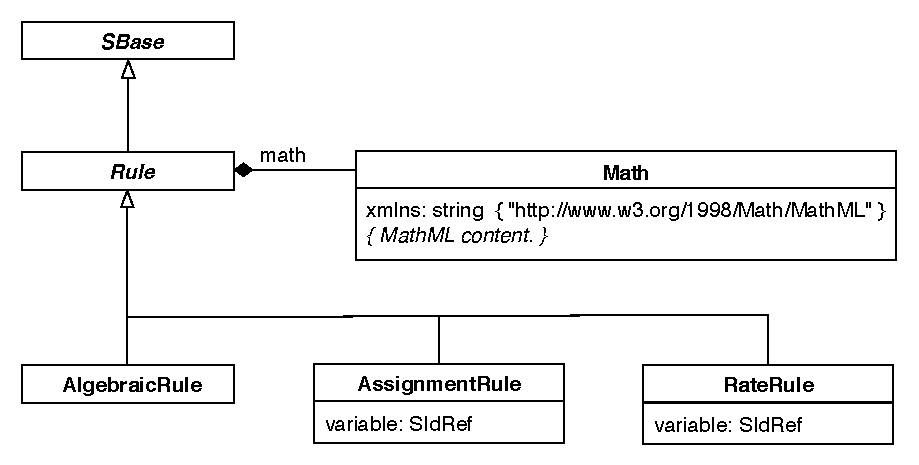
\includegraphics[scale=0.8]{figs/rule-uml}
  \caption{The definition of \Rule and derived types
      \AlgebraicRule, \AssignmentRule and \RateRule.}
  \label{fig:rules}
\vspace*{3ex}
\end{figure}



\subsubsection{Common attributes in \abstractclass{Rule}}
\label{sec:rule-math}\label{sec:rule-fields}\label{sec:rule-sboterm}

The classes derived from \Rule inherit \token{math} and
  the attributes and elements from \SBase, including
\token{sboTerm}.


\paragraph{The \token{math} element}

A \Rule object has a required element called \token{math},
containing a MathML expression defining the mathematical formula
of the rule.  This MathML formula must return a numerical value.
The formula can be an arbitrary expression referencing the
variables and other entities in an SBML model.  The interpretation
of \token{math} and the units of the formula are described in more
detail in Sections~\ref{sec:algebraicrule},
\ref{sec:assignmentrule} and~\ref{sec:raterule} below.


\paragraph{The \token{sboTerm} attribute}

\Rule inherits an optional \token{sboTerm}
attribute of type \primtype{SBOTerm} from its parent
class \SBase (see Sections~\ref{sec:sboterm-type}
and~\ref{sec:sboTerm}).  When a value is given to this
attribute in a   \AlgebraicRule, \AssignmentRule, or
\RateRule instance, it should be an
SBO identifier belonging to the branch for type  \AlgebraicRule, \AssignmentRule, or
\RateRule indicated in Table~\ref{tab:sboterm-availability}.  The relationship is
of the form ``the rule \emph{is a} X'', where X is
the SBO term.  The term chosen should be the most precise (narrow)
one that captures the role of the rule in the model.

As discussed in Section~\ref{sec:sboTerm}, SBO labels are optional
information on a model.  Applications are free to ignore
\token{sboTerm} values.  A model must be interpretable without the
benefit of SBO labels.


\subsubsection{\class{AlgebraicRule}}
\label{sec:algebraicrule}

The rule type \AlgebraicRule is used to express equations that are
neither assignments of model variables nor rates of change.
\AlgebraicRule does not add any attributes to the basic \Rule; its
role is simply to distinguish this case from the other cases.  An
example of the use of \AlgebraicRule is given in
Section~\ref{sec:algeraiceg}.

In the context of a simulation, algebraic rules are in effect at
all times, $t \geq 0$.  For purposes of evaluating expressions
that involve the \emph{delay} \token{csymbol}
(Section~\ref{sec:csymbol-token}), algebraic rules are considered
to apply also at $t \leq 0$.  Section~\ref{sec:before-t0} provides
additional information about the semantics of assignments, rules,
and entity values for simulation time $t \leq 0$.



The ability to define arbitrary algebraic expressions in an SBML
model introduces the possibility that a model is mathematically
overdetermined by the overall system of equations constructed from
its rules, reactions and events.  An SBML model must not be
overdetermined; this is discussed in
Section~\ref{sec:ruleconstraints} below.




\subsubsection{\class{AssignmentRule}}
\label{sec:assignmentrule}

The rule type \AssignmentRule is used to express equations that
set the values of variables.  The left-hand side (the
\token{variable} attribute) of an assignment rule can refer to the
identifier of a \Species, \SpeciesReference, \Compartment, 
or \Parameter object in
the model (but not a reaction).  The entity identified must not
have its \token{constant} attribute set to \val{true}.  The effects of
an \AssignmentRule are in general terms the same, but differ in
the precise details depending on the type of variable being set:

\begin{itemize}
  
\item \emph{In the case of a species}, an \AssignmentRule sets the
  referenced species' quantity (\quantity{concentration} or
  \quantity{amount of substance}) to the value determined by the
  formula in \token{math}.  The units of the formula in
  \token{math} should be the same as the \emph{units of the species}
  (Section~\ref{sec:species-units}) for the species identified by
  the \token{variable} attribute of the \AssignmentRule.
  
  \emph{Restrictions}: There must not be both an \AssignmentRule
  \token{variable} attribute and a \SpeciesReference \token{species}
  attribute having the same value, unless that species has its
  \token{boundaryCondition} attribute set to \val{true}.  In other
  words, an assignment rule cannot be defined for a species that
  is created or destroyed in a reaction unless that species is
  defined as a boundary condition in the model.

\item \emph{In the case of a species reference}, an \AssignmentRule sets
  the stoichiometry of the referenced \SpeciesReference to the value 
  determined by the formula in \token{math}.

\item \emph{In the case of a compartment}, an \AssignmentRule sets
  the referenced compartment's size to the value determined by the
  formula in \token{math}.  The overall units of the formula in
  \token{math} should be the same as the units of the size of the
  compartment (Section~\ref{sec:compartment-units}).
  
\item \emph{In the case of a parameter}, an \AssignmentRule sets
  the referenced parameter's value to that determined by the
  formula in \token{math}.  The overall units of the formula in
  \token{math} should be the same as the units defined for the
  parameter (Section~\ref{sec:parameter-units}).

\end{itemize}

In the context of a simulation, assignment rules are in effect at
all times, $t \geq 0$.  For purposes of evaluating expressions
that involve the \emph{delay} \token{csymbol}
(Section~\ref{sec:csymbol-token}), assignment rules are considered
to apply also at $t \leq 0$.  Section~\ref{sec:before-t0} provides
additional information about the semantics of assignments, rules,
and entity values for simulation time $t \leq 0$.

A model must not contain more than one \AssignmentRule or
\RateRule object having the same value of \token{variable}; in
other words, in the set of all assignment rules and rate rules in
an SBML model, each variable appearing in the left-hand sides can
only appear once.  This simply follows from the fact that an
indeterminate system would result if a model contained more than
one assignment rule for the same variable or both an assignment
rule and a rate rule for the same variable.

Similarly, a model must also not contain \emph{both} an
\AssignmentRule and an \InitialAssignment for the same variable,
because both kinds of constructs apply prior to and at the start
of simulation time, \ie $t \leq 0$.  If a model contained both an
initial assignment and an assignment rule for the same variable,
an indeterminate system would result.  (See also
Section~\ref{sec:initial-assignment-semantics}.)

The value calculated by an \AssignmentRule object overrides the
value assigned to the given symbol by the object defining that
symbol.  For example, if a \Compartment's \token{size} is set in
its definition, and the model also contains an \AssignmentRule
having that compartment's \token{id} as its \token{variable}
value, then the \token{size} assigned in the \Compartment
definition is ignored and the value assigned based on the
computation defined in the \AssignmentRule.  This does \emph{not}
mean that a definition for a given symbol can be omitted if there
is an \AssignmentRule object for it.  For example, there must be a
\Parameter definition for a given parameter if there is an
\AssignmentRule for that parameter.


\subsubsection{\class{RateRule}}
\label{sec:raterule}

The rule type \RateRule is used to express equations that
determine the rates of change of variables.  The left-hand side
(the \token{variable} attribute) can refer to the identifier of a
species, species reference, compartment, or parameter (but not a 
reaction).  The
entity identified must have its \token{constant} attribute set to
\val{false}.  The effects of a \RateRule are in general terms the
same, but differ in the precise details depending on which
variable is being set:

\begin{itemize}
  
\item \emph{In the case of a species}, a \RateRule sets the rate
  of change of the species' quantity (\quantity{concentration} or
  \quantity{amount of substance}) to the value determined by the
  formula in \token{math}.  The overall units of the formula in
  \token{math} should be \quantity{species
    quantity}/\quantity{time}, where the \quantity{time} units are
  the predefined units of time described in
  Section~\ref{sec:unitdefinitions} and the \quantity{species
    quantity} units are the \emph{units of the species} as defined
  in Section~\ref{sec:species-units}.
  
  \emph{Restrictions}: There must not be both a \RateRule
  \token{variable} attribute and a \SpeciesReference \token{species}
  attribute having the same value, unless that species has its
  \token{boundaryCondition} attribute is set to \val{true}.  This
  means a rate rule cannot be defined for a species that is
  created or destroyed in a reaction, unless that species is
  defined as a boundary condition in the model.
  
\item \emph{In the case of a species reference}, a \RateRule sets the rate
  of change of the \SpeciesReference's stoichiometry value to that 
  determined by the formula in \token{math}.  
  
\item \emph{In the case of a compartment}, a \RateRule sets the
  rate of change of the compartment's size to the value determined
  by the formula in \token{math}.  The overall units of the
  formula should be \quantity{size}/\quantity{time}, where the
  \quantity{time} units are the predefined units of time described
  in Section~\ref{sec:unitdefinitions} and the \quantity{size}
  units are the units of size on the compartment
  (Section~\ref{sec:compartment-units}).

\item \emph{In the case of a parameter}, a \RateRule sets the rate
  of change of the parameter's value to that determined by the
  formula in \token{math}.  The overall units of the formula should
  be \quantity{x}/\quantity{time}, where \quantity{x} are the
  units of the parameter (Section~\ref{sec:parameter-units}).

\end{itemize}

In the context of a simulation, rate rules are in effect for
simulation time $t > 0$.  Other types of rules and initial
assignments are in effect at different times;
Section~\ref{sec:before-t0} describes these conditions.

As mentioned in Section~\ref{sec:assignmentrule} for
\AssignmentRule, a model must not contain more than one \RateRule
or \AssignmentRule object having the same value of
\token{variable}; in other words, in the set of all assignment
rules and rate rules in an SBML model, each variable appearing in
the left-hand sides can only appear once.  This simply follows
from the fact that an indeterminate system would result if a model
contained more than one assignment rule for the same variable or
both an assignment rule and a rate rule for the same variable.


\subsubsection{Additional restrictions on rules}
\label{sec:ruleconstraints}

An important design goal of SBML rule semantics is to ensure that
a model's simulation and analysis results will not be dependent on
when or how often rules are evaluated.  To achieve this, SBML
needs to place two additional restrictions on rule use in addition
to the conditions described above regarding the use of
\AlgebraicRule, \AssignmentRule and \RateRule.  The first concerns
algebraic loops in the system of assignments in a model, and the
second concerns overdetermined systems.


\paragraph{The model must not contain algebraic loops}

The combined set of \InitialAssignment, \AssignmentRule and
\KineticLaw objects constitute a set of assignment statements that
should be considered as a whole.  (A \KineticLaw object is counted
as an assignment because it assigns a value to the symbol
contained in the \token{id} attribute of the \Reaction object in which
it is defined.)  This combined set of assignment statements must
not contain algebraic loops---dependency chains between these
statements must terminate.  To put this more formally, consider a
directed graph in which nodes are assignment statements and
directed arcs exist for each occurrence of an SBML species, species reference,
compartment or parameter symbol in an assignment statement's
\token{math} element.  Let the directed arcs point from the
statement assigning the symbol to the statements that contain the
symbol in their \token{math} element expressions.  This graph must
be acyclic.

SBML does not specify when or how often rules should be evaluated.
Eliminating algebraic loops ensures that assignment statements can
be evaluated any number of times without the result of those
evaluations changing.  As an example, consider the following
equations:
\begin{linenomath}
\begin{equation*}
  \begin{array}{lll}
    x = x + 1, & y = z + 200, & z = y + 100
  \end{array}
\end{equation*}
\end{linenomath}
If this set of equations were interpreted as a set of assignment
statements, it would be invalid because the rule for $x$ refers to
$x$ (exhibiting one type of loop), and the rule for $y$ refers to
$z$ while the rule for $z$ refers back to $y$ (exhibiting another
type of loop).

Conversely, the following set of equations would constitute a
valid set of assignment statements:
\begin{linenomath}
\begin{equation*}
  \begin{array}{lll}
    x = 10, & y = z + 200, & z = x + 100
  \end{array}
\end{equation*}
\end{linenomath}


\paragraph{The model must not be overdetermined}

An SBML model must not be overdetermined; that is, a model must
not define more equations than there are unknowns in a model.  An
SBML model that does not contain \AlgebraicRule objects cannot
be overdetermined.

Assessing whether a given continuous, deterministic, mathematical
model is overdetermined does not require dynamic analysis; it can
be done by analyzing the system of equations created from the
model.  It should be noted that where a model contains both
reactions and events there are several sets of equations to
consider when determining whether a model is overdetermined.  The
set of equations derived from the combined set of rules and 
reactions and, for each event, the set of equations derived from
the combined set of rules and event assignments for the particular
event. 

One approach is to construct a bipartite graph in which
one set of vertices represents the variables and the other the set
of vertices represents the equations.  Place edges between
vertices such that variables in the system are linked to the
equations that determine them.  A mathematical model is 
overdetermined if the maximal matchings~\citep{chartrand_1977} 
of the bipartite graph contain disconnected vertexes representing 
equations.  (If one maximal matching has this property, then all the 
maximal matchings will have this property; \ie it is only necessary 
to find one maximal matching.)  
Appendix~\ref{apdx:assessing-overdetermined} describes
a method of applying this procedure to specific SBML data objects.
In some cases it is possible to avoid the use of an \AlgebraicRule. 
This is discussed in more detail in Section~\ref{sec:bp:rules}.


\subsubsection{Example of rule use}
\label{sec:eg-rule-use}

This section contains an example set of rules.  Consider the
following set of equations:
\begin{linenomath}
  \begin{equation*}
    \begin{array}{lll}
      k = \dfrac{k_3}{k_2}, & s_2 = \dfrac{k \cdot x}{1 + k_2}, & A = 0.10 \cdot x
    \end{array}
  \end{equation*}
\end{linenomath}
This can be encoded by the following scalar rule set (where the
definitions of \texttt{x}, \texttt{s}, \texttt{k}, \texttt{k2},
\texttt{k3} and \texttt{A} are assumed to be located elsewhere in
the model and not shown in this abbreviated example):

\begin{example}
    <listOfRules>
        <assignmentRule variable="k">
            <math xmlns="http://www.w3.org/1998/Math/MathML">
                <apply> <divide/> <ci> k3 </ci> <ci> k2 </ci> </apply>
            </math>
        </assignmentRule>
        <assignmentRule variable="s2">
            <math xmlns="http://www.w3.org/1998/Math/MathML">
                <apply>
                    <divide/>
                        <apply> <times/> <ci> k </ci> <ci> x </ci> </apply>
                        <apply> <plus/> <cn> 1 </cn> <ci> k2 </ci> </apply>
                </apply>
            </math>
        </assignmentRule>
        <assignmentRule variable="A">
            <math xmlns="http://www.w3.org/1998/Math/MathML">
                <apply> <times/> <cn> 0.10 </cn> <ci> x </ci> </apply>
            </math>
        </assignmentRule>
    </listOfRules>
\end{example}


%\subsubsection{Guidelines for Evaluating Rules}
%
%This section describes how rules including those implied by
%\Reaction structures (see Section~\ref{sec:reactions})
%should be evaluated.  For the purpose of interpreting models
%mathematically (and for this description), \Reaction
%structures collectively imply a \class{SpeciesConcentrationRule}
%structure, of type \class{rate}, for each species referenced in a
%\SpeciesReference structure excluding those species which
%are defined with the \token{boundaryCondition} attribute equal to
%\texttt{true}.
%
%To determine the initial values of variables is a 2 set process:
%
%\begin{itemize}
%
%\item variables should be set according to the initial values
%given by \Species, \Compartment and
%\Parameter structures then
%
%\item the \class{scalar} rules should be evaluated
%
%\end{itemize}
%
%To determine the rates of change of variables given a set of
%current variable values is again a two set process:
%
%\begin{itemize}
%
%\item the \class{scalar} rules should be evaluated then
%
%\item the \class{rate} rules should be evaluated
%
%\end{itemize}
%
%The \class{scalar} rules should be evaluated to determine the
%complete set of variable values given an incomplete set of
%variable values determined by \class{rate} and
%\AlgebraicRule structures.
%


%-----------------------------------------------------------------------------
\subsection{Constraints}
\label{sec:constraints}
%-----------------------------------------------------------------------------

The \Constraint object is a mechanism for stating the
assumptions under which a model is designed to operate.  The
\emph{constraints} are statements about permissible values of
different quantities in a model.  Figure~\ref{fig:constraint}
shows the definition of the \Constraint object class.

\begin{figure}[htb]
  \centering
  \small
  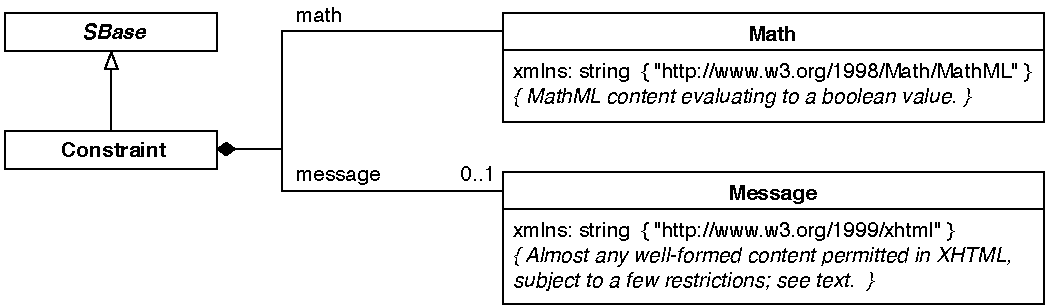
\includegraphics[scale=0.8]{figs/constraint-uml}
  \caption{The definition of class \Constraint.  The
      contents of the \class{Math} class can be any \mathml
      permitted in SBML, but it must return a boolean value.  As
      shown above, an instance of \Constraint can also contain
      zero or one instances of \class{Message}; this element is
      simply a wrapper (in the XML form, within \token{<message>
        \ldots{} </message>} tags) for XHTML content.  The same
      guidelines for XHTML content as explained in
      Section~\ref{sec:notes} for notes on \SBase also apply to
      the XHTML within messages in a \Constraint. A sequence of
      one or more instances of \Constraint objects can be located
      in an instance of \ListOfConstraints in \Model, as shown in
      Figure~\protect\ref{fig:model}.}
  \label{fig:constraint}
\end{figure}

The essential meaning of a constraint is this: if a dynamical
analysis of a model (such as a simulation) reaches a state in
which a constraint is no longer satisfied, the results of the
analysis are deemed invalid beginning with that point in time.
The exact behavior of a software tool, upon encountering a
constraint violation, is left up to the software; \emph{however},
a software tool must somehow indicate to the user when a model's
constraints are no longer satisfied.  (Otherwise, a user may not
realize that the analysis has reached an invalid state and is
potentially producing nonsense results.)  If a software tool does
not have support for constraints, it should indicate this to the
user when encountering a model containing constraints.


\subsubsection{The \token{math} element}

\Constraint has one required subelement, \token{math},
containing a MathML formula defining the condition of the
constraint.  This formula must return a boolean value of
\val{true} when the model is in a \emph{valid} state.  The formula
can be an arbitrary expression referencing the variables and other
entities in an SBML model.  The evaluation of \token{math} and
behavior of constraints are described in more detail in
Section~\ref{sec:constraint-semantics} below.


\subsubsection{The \token{message} element}
\label{sec:constraint-message}

A \Constraint object has an optional element called
\token{message}.  This can contain a message in XHTML format that
may be displayed to the user when the condition of the constraint
in \token{math} evaluates to a value of \val{false}.  Software
tools are not required to display the message, but it is
recommended that they do so as a matter of best practice.

The XHTML content within a \token{message} element must follow the
same restrictions as for the \token{notes} element on \SBase
described in Section~\ref{sec:notes}.  For example,
\token{message} must not contain an XML declaration or a DOCTYPE
declaration, and the permitted content can only take one of the
following general forms: (1) a complete XHTML document beginning
with the element \token{<html>} and ending with \token{</html>};
(2) the ``body'' portion of a document beginning with the element
\token{<body>} and ending with \token{</body>}; or (3) XHTML
content that is permitted within a \token{<body>} ...
\token{</body>} elements.    Appendix~\ref{apdx:processing-notes}
describes one approach to reading the \token{message} content.


\subsubsection{The \token{sboTerm} attribute}
\label{sec:constraint-sboterm}

\Constraint inherits an optional \token{sboTerm}
attribute of type \primtype{SBOTerm} from its parent
class \SBase (see Sections~\ref{sec:sboterm-type}
and~\ref{sec:sboTerm}).  When a value is given to this
attribute in a  \Constraint instance, it should be an
SBO identifier belonging to the branch for type  \Constraint
indicated in Table~\ref{tab:sboterm-availability}.  The relationship is
of the form ``the constraint \emph{is a} X'', where X is
the SBO term.  The term chosen should be the most precise (narrow)
one that captures the role of the constraint in the model.

As discussed in Section~\ref{sec:sboTerm}, SBO labels are optional
information on a model.  Applications are free to ignore
\token{sboTerm} values.  A model must be interpretable without the
benefit of SBO labels.


\subsubsection{Semantics of constraints}
\label{sec:constraint-semantics}

In the context of a simulation, a \Constraint has effect at all
times $t \geq 0$.  Each \Constraint's \token{math} element is first
evaluated after any \InitialAssignment definitions in a model at
$t = 0$ and can conceivably trigger at that point.  (In other
words, a simulation could fail a constraint immediately.)

\Constraint definitions \emph{cannot and should not} be used to
compute the dynamical behavior of a model as part of, for example,
simulation.  Constraints may be used as input to non-dynamical
analysis, for instance by expressing flux constraints for flux
balance analysis.

The results of a simulation of a model containing a constraint are
invalid from any simulation time at and after a point when the
function given by the \token{math} returns a value of \val{false}.
Invalid simulation results do not make a prediction of the
behavior of the biochemical reaction network represented by the
model.  The precise behavior of simulation tools is left undefined
with respect to constraints.  If invalid results are detected with
respect to a given constraint, the \token{message} element
(Section~\ref{sec:constraint-message}) may optionally be displayed
to the user.  The simulation tool may also halt the simulation or
clearly delimit in output data the simulation time point at which
the simulation results become invalid.

SBML does not impose restrictions on duplicate \Constraint
definitions or the order of evaluation of \Constraint objects in a
model.  It is possible for a model to define multiple constraints
all with the same \token{math} element.  Since the failure of any
constraint indicates that the model simulation has entered an
invalid state, a system is not required to attempt to detect
whether other constraints in the model have failed once any one
constraint has failed.


\subsubsection{Example}

As an example, the following SBML fragment demonstrates the
constraint that species $S_1$ should only have values between 1
and 100:

\begin{example}
<model>
    ...
    <listOfConstraints>
        <constraint>
            <math xmlns="http://www.w3.org/1998/Math/MathML">
                <apply>
                    <and/>
                        <apply> <lt/> <cn> 1 </cn> <ci> S1 </ci> </apply>
                        <apply> <lt/> <ci> S1 </ci> <cn> 100 </cn> </apply>
                </apply>
            </math>
            <message>
                <p xmlns="http://www.w3.org/1999/xhtml"> Species S1 is out of range. </p>
            </message>
        </constraint>
    </listOfConstraints>
    ...
</model>
\end{example}


%-----------------------------------------------------------------------------
\subsection{Reactions}
\label{sec:reactions}
%-----------------------------------------------------------------------------

A \emph{reaction} represents any transformation, transport or
binding process, typically a chemical reaction, that can change
the quantity of one or more species. 
To describe a reaction in SBML it is necessary to define its \emph{structural}
properties, i.e. the participating reactants and products (and their 
corresponding stoichiometries) and its reversibility. 
In addition there can be a \emph{quantitative} description of the rate of the
reaction, consisting mainly of a list of additional modifier species that 
have an influence on the reaction rate and a mathematical rate law 
including optional parameters.
Some software tools will interprete only the structural part of the reactions
in an SBML model, but tools doing simulations or numerical analysis will
usually also consider the quantitative information.
The various parts of a
reaction are recorded in the SBML \Reaction object class and other
supporting data classes, defined in Figure~\vref{fig:reaction}.

\begin{figure}[htb]
  \centering
  \vspace*{2ex}
  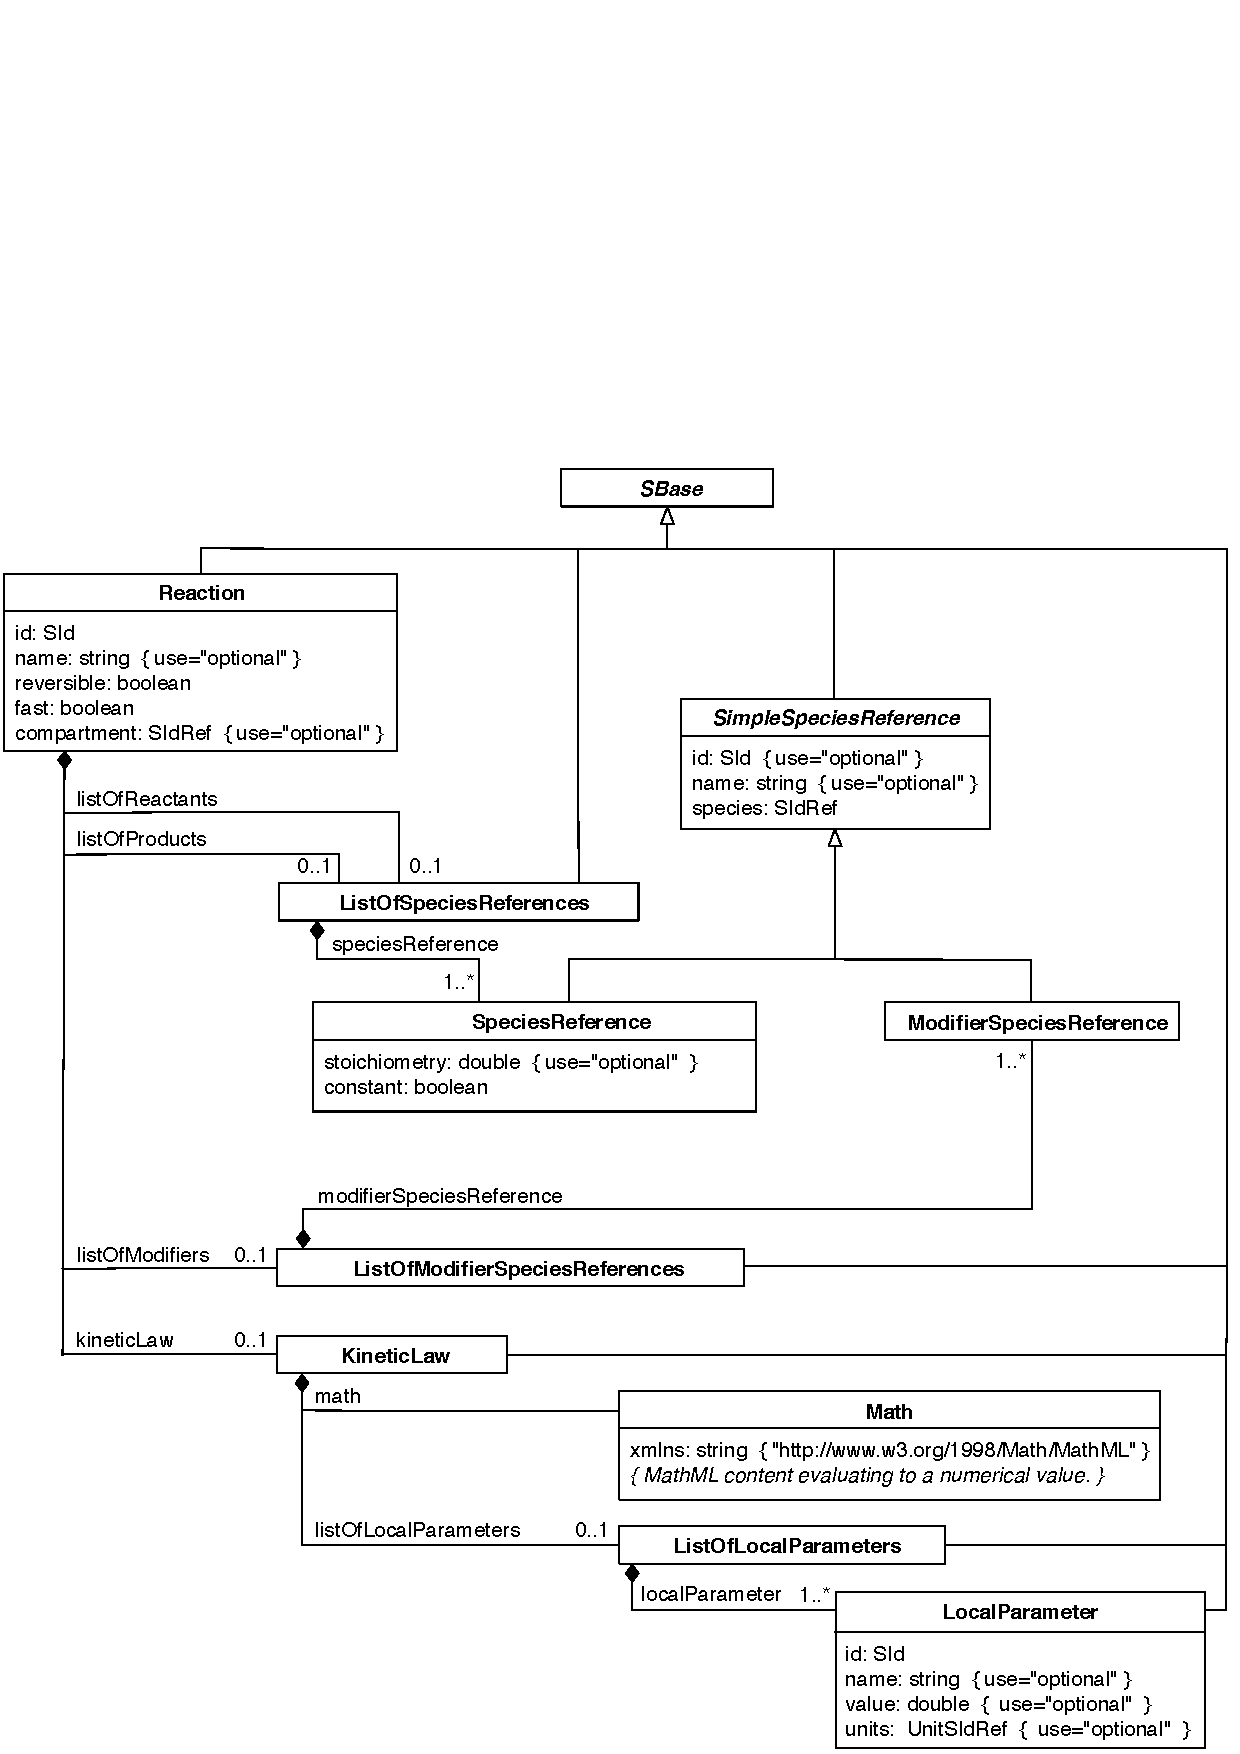
\includegraphics[scale=0.8]{figs/reaction-uml-v2}
  \vspace*{0.5ex}
  \caption{The definitions of classes \Reaction, \KineticLaw,
      \SpeciesReference, \ModifierSpeciesReference, \LocalParameter,
      as well as the
      container classes \ListOfReactants, \ListOfProducts,
      \ListOfModifiers, and \ListOfLocalParameters.  Note that
      \SimpleSpeciesReference is an abstract class used only to
      provide some common attributes to its derived classes.}
  \label{fig:reaction}
\end{figure}


\subsubsection{\class{Reaction}}
\label{sec:reaction-type}
\label{sec:listofreactants}
\label{sec:listofproducts}
\label{sec:listofmodifiers}

Each reaction in an SBML model is defined using an instance of a
\Reaction object.  As shown in Figure~\vref{fig:reaction}, it
contains several scalar attributes and several lists of objects.


\paragraph{The \token{id} and \token{name} attributes}

As with most other main kinds of objects in SBML, the
\Reaction object class
includes a mandatory attribute called \token{id}, of type
\primtype{SId}, and an optional attribute \token{name}, of type
\primtype{string}.  The \token{id} attribute is used to give the
reaction a unique identifier in the model.  This identifier can be
used in mathematical formulas elsewhere in an SBML model to
represent the rate of that reaction; this usage is explained in
detail in Section~\ref{subsec:reaction-as-symbol} below.  The
\token{name} attribute can be used to give the reaction a more
free-form, descriptive name.  The \token{name} and \token{id}
attributes must be used as described in
Section~\ref{sec:idnameattribs}.


\paragraph{The lists of reactants, products and modifiers}

The species participating as reactants, products, and/or modifiers
in a reaction are declared using lists of \SpeciesReference and/or
\ModifierSpeciesReference instances stored in
\token{listOfReactants}, \token{listOfProducts} and
\token{listOfModifiers}.
\SpeciesReference and
\ModifierSpeciesReference are described in more detail
in Sections~\ref{subsec:speciesreference}
and~\ref{subsec:modifierreference} below.

Certain restrictions are placed on the appearance of species in
reaction definitions:
\begin{itemize}
  
\item The ability of a species to appear as a reactant or product
  of any reaction in a model is governed by certain flags in that
  species' definition; see Section~\ref{sec:species-constant} for
  more information.
  
\item Any species appearing in the mathematical formula of the
  \token{kineticLaw} of a \Reaction instance must be declared in
  at least one of that \Reaction's lists of reactants, products,
  and/or modifiers.  Put another way, it is an error for a
  reaction's kinetic law formula to refer to species that have not
  been declared for that reaction.
  
\item A reaction definition can contain an empty list of reactants
  \emph{or} an empty list of products, but it must have at least
  one reactant or product; in other words, a reaction without any
  reactant or product species is not permitted.  (This restriction
  does not apply to modifier species, which remain optional in all
  cases.)

\end{itemize}


\paragraph{The \token{kineticLaw} element}

A reaction can contain up to one \KineticLaw object in the
\token{kineticLaw} element of the \Reaction.  This ``kinetic law''
defines the speed at which the process defined by the reaction
takes place.  A detailed description of \KineticLaw is left to
Section~\ref{subsec:kinetic-law} below.

Note that the inclusion of a \KineticLaw object in an instance
of a \Reaction component is optional; however, missing rate laws mean
that a lot of techniques for numerical analysis and simulation of the 
model will not be applicable. 
Nevertheless, for some modeling applications,
reactions without any defined rate can be perfectly acceptable.


\paragraph{The \token{reversible} attribute}
\label{sec:reversible}

The mandatory boolean attribute \token{reversible} indicates whether
the reaction is reversible.  

To say that a reaction is \emph{reversible} is to say it can
proceed in either the forward or the reverse direction.
This information may be redundant in cases where the reversibility of the 
reaction can be deduced by inspecting its rate expression. However, a reaction
is not required to have a rate law and if the rate law is present it may not
always be possible to deduce the reversibility from it. 
Having a separate attribute allows certain kinds of structural analysis such as 
elementary mode analysis even in these cases.

Mathematically, the \token{reversible} attribute on \Reaction has no impact on 
the construction of the equations for change of the species quantities. However, 
labeling a reaction as irreversible would be interpreted as an assertion that 
the rate law will not have negative values during a simulation. 
Software tools could provide a means of testing that this condition holds.  
The presence of reversibility information in two places (\ie the rate expression
and the \token{reversible} flag) leaves open the possibility that
a model could contain contradictory information, but this would be considered as
a problem of the encoded model rather than as an invalid SBML encoding.

\paragraph{The \token{fast} attribute}
\label{sec:fast}

The optional boolean attribute \token{fast} is another required
boolean attribute of \Reaction.  

When a model contains a true value for \token{fast} on any of its
reactions, it indicates that the creator of the model is
distinguishing different time scales of reactions in the system.
If a model does not distinguish between time scales the \token{fast} 
attribute should be set to \val{false} for all reactions. 

The model's reaction definitions are divided into two sets by the
values of the \token{fast} attributes.  The set of reactions having
\token{fast}=\val{true} (known as \emph{fast reactions}) should be
assumed to be operating on a time scale significantly faster than
the other reactions (the \emph{slow reactions}).  Fast reactions
are considered to be instantaneous relative to the slow reactions.
Software tools should use a pseudo steady-state approximation for
the set of fast reactions when constructing the system of
equations for the model.  More specifically, the set of reactions
that have the \token{fast} attribute set to \val{true} forms a
subsystem that should be described by a pseudo steady-state
approximation in relationship to all other reactions in the model.
Under this description, relaxation from any initial condition or
perturbation from any intermediate state of this subsystem would
be infinitely fast.
Appendix~\ref{apdx:consequences-of-being-fast} provides a
technical explanation of an approach to solving systems with fast
reactions.

The correctness of the approximation requires a significant
separation of time scales between the fast reactions and other
processes.  It is the responsibility of the modeler or of the software tool
writing the SBML file to ensure this condition is fulfilled.

Note that the \token{fast} flag has significant effect on the mathematical
interpretation of a model and cannot be safely ignored if a software 
tool does not implement support for the corresponding concept. 

\paragraph{The \token{compartment} attribute on \class{Reaction}}
\label{sec:reaction-compartment}

The optional attribute \token{compartment} of type \primtype{SIdRef} 
can be used to indicate a compartment in which the reaction takes place. 
If the attribute is present its value must be the identifier of a 
compartment defined in the enclosing \Model. 

Similar to the \token{reversible} attribute the value of the \token{compartment} 
attribute has no direct implication on the construction of the
mathematical equations. However, tools may make use of this information 
to analyze the structure of the model, to guide the modeler in choosing 
the correct rate law, or for visualization purposes.  

\paragraph{The \token{sboTerm} attribute on \class{Reaction}}
\label{sec:reaction-sboterm}

\Reaction inherits an optional \token{sboTerm}
attribute of type \primtype{SBOTerm} from its parent
class \SBase (see Sections~\ref{sec:sboterm-type}
and~\ref{sec:sboTerm}).  When a value is given to this
attribute in a  \Reaction instance, it should be an
SBO identifier belonging to the branch for type  \Reaction  
indicated in Table~\ref{tab:sboterm-availability}.  The relationship is
of the form ``the reaction \emph{is a} X'', where X is
the SBO term.  The term chosen should be the most precise (narrow)
one that captures the role of the reaction in the model.

As discussed in Section~\ref{sec:sboTerm}, SBO labels are optional
information on a model.  Applications are free to ignore
\token{sboTerm} values.  A model must be interpretable without the
benefit of SBO labels.

\subsubsection{The \class{SimpleSpeciesReference} abstract type}
\label{subsec:simplespeciesreference}

As mentioned above, every species that enters into a given
reaction must appear in that reaction's lists of reactants,
products and/or modifiers.  In an SBML model, all species that may
participate in any reaction are listed in the
\token{listOfSpecies} element of the top-level \Model instance
(see Section~\ref{sec:model}).  Lists of products, reactants and
modifiers in \Reaction objects do not introduce new species,
but rather, they refer back to those listed in the model's
top-level \token{listOfSpecies}.  For reactants and products, the
connection is made using a \SpeciesReference object; for
modifiers, it is made using a \ModifierSpeciesReference 
object.  \SimpleSpeciesReference, defined in
Figure~\vref{fig:reaction}, is an abstract type that serves as the
parent class of both \SpeciesReference and
\ModifierSpeciesReference.  It is used simply to hold the attributes
and elements that are common to the latter two objects.


\paragraph{The \token{id} and \token{name} attributes}

The optional identifier stored in the \token{id} attribute  of type
\primtype{SId} allows \SpeciesReference and \ModifierSpeciesReference 
instances to be referenced from other objects. The \token{id} value 
(whether it is in a \SpeciesReference or \ModifierSpeciesReference object) 
exists in the global namespace of the model.   A
\SpeciesReference or \ModifierSpeciesReference can also have an 
optional \token{name} attribute of type
\primtype{string}.The \token{id} and \token{name}
attributes must be used as described in
Section~\ref{sec:idnameattribs}.


\paragraph{The \token{species} attribute}

The \SimpleSpeciesReference object class has a required attribute,
\token{species}, of type \primtype{SIdRef}.  As with the other
attributes, it is inherited by \SpeciesReference and
\ModifierSpeciesReference.  The value of \token{species} must be the
identifier of a species defined in the enclosing \Model.  The
species is thereby declared as participating in the reaction being
defined.  The precise role of that species as a reactant, product,
or modifier in the reaction is determined by the subtype of
\SimpleSpeciesReference (\ie either \SpeciesReference or
\ModifierSpeciesReference) in which the identifier appears and by the 
specific list of species references in which the \SpeciesReference appears.


\paragraph{The \token{sboTerm} attribute}
\label{sec:simplespeciesreference-sboterm}

\SimpleSpeciesReference inherits an optional \token{sboTerm}
attribute of type \primtype{SBOTerm} from its parent
class \SBase (see Sections~\ref{sec:sboterm-type}
and~\ref{sec:sboTerm}).  When a value is given to this
attribute in a  \SimpleSpeciesReference instance, it should be an
SBO identifier belonging to the branch for type  \SimpleSpeciesReference 
indicated in Table~\ref{tab:sboterm-availability}.  The relationship is
of the form ``the species reference \emph{is a} X'', where X is
the SBO term.  The term chosen should be the most precise (narrow)
one that captures the role of the species reference in the model.

As discussed in Section~\ref{sec:sboTerm}, SBO labels are optional
information on a model.  Applications are free to ignore
\token{sboTerm} values.  A model must be interpretable without the
benefit of SBO labels.

\subsubsection{\class{SpeciesReference}}
\label{subsec:speciesreference}

The \Reaction object class provides a way to express which species
act as reactants and which species act as products in a reaction.
In a given reaction, references to those species acting as
reactants and/or products are made using instances of
\SpeciesReference objects in \Reaction's lists of reactants and
products.  The \SpeciesReference structure inherits the mandatory
attribute \token{species} and optional attributes \token{id},
\token{name}, and \token{sboTerm}, from the parent type
\SimpleSpeciesReference; see
Section~\ref{subsec:simplespeciesreference} for their definitions.
It also defines the optional attribute \token{stoichiometry} and 
the mandatory attribute \token{constant}, described below.

The \token{species} attribute value must be the
identifier of an existing species defined in the enclosing \Model;
the species is thereby designated as a reactant or product in the
reaction.  Which one it is (\ie reactant or product) is indicated
by whether the \SpeciesReference appears in the \Reaction's
\token{reactant} or \token{product} lists.


\paragraph{The \token{stoichiometry} attribute}

The {\em stoichiometry} of a species in a reaction describes how much 
the value of the species changes when the reaction takes place, \ie 
how much of the reactants is consumed and how much of the products is produced.
Product and reactant stoichiometries are specified using
the optional \token{stoichiometry} attribute 
in a \SpeciesReference object.  The \token{stoichiometry}
attribute is of type double and should contain values greater than
zero (0). 

A missing \token{stoichiometry} implies that the stoichiometry is either unknown, 
or to be obtained from an external source, or determined by an initial
assignment (Section~\ref{sec:initialAssignment}) or a rule
(Section~\ref{sec:rules}) elsewhere in the model.

A species reference's stoichiometry is set by its \token{stoichiometry} 
attribute exactly once.  If the species reference's \token{constant} 
attribute has the value
\val{true}, then the stoichiometry is fixed and cannot be
changed except by an \InitialAssignment.  These two methods of
setting the stoichiometry differ in that the \token{stoichiometry}
attribute can only be used to set it to a literal scalar value,
whereas \InitialAssignment allows the stoichiometry to be set using an
arbitrary mathematical expression.  If the species reference's
\token{constant} attribute has the value \val{false}, the species reference's
value may be overridden by an \InitialAssignment or changed by
\AssignmentRule or \AlgebraicRule, and in addition, for simulation
time $t > 0$, it may also be changed by a \RateRule or \Event{}s.
(However, some of these constructs are mutually exclusive; see
Sections~\ref{sec:rules} and~\ref{sec:events}.)  It is not an
error to define \token{stoichiometry} on a species reference and also 
redefine the stoichiometry using an \InitialAssignment, but the 
\token{stoichiometry} attribute in that case is ignored.  
Section~\ref{sec:before-t0} provides additional
information about the semantics of assignments, rules and values
for simulation time $t \leq 0$.

An explanation of how exactly the stoichiometry is used in the mathematical interpretation 
of the model is given in Section~\ref{sec:about-kinetic-laws}.


\paragraph{The \token{constant} attribute}

The \SpeciesReference object has a mandatory boolean attribute named
\token{constant} which indicates whether the stoichiometry can
vary during a simulation. A value \val{true} for this attribute means that 
the stoichiometry of the referenced species takes the value of the 
\token{stoichiometry} attribute, unless it is changed by an \InitialAssignment.
A value of \val{false} indicates the stoichiometry 
can be changed by rules (see Section~\ref{sec:rules}) and
that the value of the \token{stoichiometry} attribute is actually intended to be the initial
value of the stoichiometry.

\paragraph{Use of species reference identifiers in mathematical expressions}

The value of the \token{id} attribute of a \SpeciesReference can be
used as the content of a \token{ci} element in MathML formulas
elsewhere in the model. Such a \token{ci} element or symbol
represents the stoichiometry of the given species in the given reaction.

Furthermore, the \token{id} attribute of a \SpeciesReference can be
used in the \token{variable} attribute of an \InitialAssignment, \RateRule,
\AssignmentRule or \EventAssignment object, providing a way to describe
variable stoichiometries. This is only allowed if the 
\token{constant} attribute is set to false. 


\paragraph{Examples}

The following is a simple example of a species reference for
species \val{X0}, with stoichiometry \val{2}, in a list of
reactants within a reaction having the identifier \val{J1}:

\begin{example}
<model>
    ...
    <listOfReactions>
        <reaction id="J1" reversible="false" fast="false">
            <listOfReactants>
                <speciesReference species="X0" stoichiometry="2" constant="true"/>
            </listOfReactants>
            ...
        </reaction>
        ...
    </listOfReactions>
    ...
</model>
\end{example}

The following is a more complex example of a species reference with an id ``sr01'' and 
an initial assignment that specifies a rational number for the stoichiometry:


\begin{example}
<model>
    ...
    <listOfInitialAssignments>
        <initialAssignment symbol="sr01">
            <math xmlns="http://www.w3.org/1998/Math/MathML">
                <cn type="rational"> 3 <sep/> 2 </cn>
            </math>
        </initialAssignment>
        ...
    </listOfInitialAssignments>
	...
    <listOfReactions>
        <reaction id="J1" reversible="true" fast="false">
            <listOfReactants>
                <speciesReference id="sr01" species="X0" constant="true"/>
            </listOfReactants>
            ...
        </reaction>
        ...
    </listOfReactions>
    ...
</model>
\end{example}


A species can occur more than once in the lists of reactants and
products of a given \Reaction instance.  The effective
stoichiometry for a species in a reaction is the sum of the
stoichiometry values given in the \SpeciesReference objects in
the list of products minus the sum of stoichiometry values given
in the \SpeciesReference objects in the list of reactants.  A
positive value indicates the species is effectively a product and
a negative value indicates the species is effectively a reactant.
SBML places no restrictions on the effective stoichiometry of a
species in a reaction; for example, it can be zero.  In the
following SBML fragment, the two reactions have the same effective
stoichiometry for all their species:

\begin{example}
<reaction id="x" reversible="false" fast="false">
    <listOfReactants>
        <speciesReference species="a" stoichiometry="1" constant="true"/>
        <speciesReference species="a" stoichiometry="1" constant="true"/>
        <speciesReference species="b" stoichiometry="1" constant="true"/>
    </listOfReactants>
    <listOfProducts>
        <speciesReference species="c" stoichiometry="1" constant="true"/>
        <speciesReference species="b" stoichiometry="1" constant="true"/>
    </listProducts>
</reaction>
<reaction id="y" reversible="false" fast="false">
    <listOfReactants>
        <speciesReference species="a" stoichiometry="2" constant="true"/>
    </listOfReactants>
    <listOfProducts>
        <speciesReference species="c" stoichiometry="1" constant="true"/>
    </listProducts>
</reaction>
\end{example}



\subsubsection{\class{ModifierSpeciesReference}}
\label{subsec:modifierreference}

Sometimes a species appears in the kinetic rate formula of a
reaction but is itself neither created nor destroyed in that
reaction (for example, because it acts as a catalyst or
inhibitor).  In SBML, all such species are simply called
\emph{modifiers} without regard to the detailed role of those
species in the model.  The \Reaction object class provides a way to
express which species act as modifiers in a given reaction.  This
is the purpose of the list of modifiers available in \Reaction.
The list contains instances of \ModifierSpeciesReference
object.

As shown in Figure~\vref{fig:reaction}, the
\ModifierSpeciesReference class inherits the mandatory attribute
\token{species} and optional attributes \token{id} and \token{name}
from the parent class \SimpleSpeciesReference; see
Section~\ref{subsec:simplespeciesreference} for their precise
definitions.

The value of the \token{species} attribute must be the identifier of a
species defined in the enclosing \Model; this species is
designated as a modifier for the current reaction.  A reaction may
have any number of modifiers.  It is permissible for a modifier
species to appear simultaneously in the list of reactants and
products of the same reaction where it is designated as a
modifier, as well as to appear in the list of reactants, products
and modifiers of other reactions in the model.

\subsubsection{\class{LocalParameter}}
\label{subsec:localparameter}

The kinetic law of a \Reaction can contain a list of local parameters that
are only used by the rate law of this specific reaction. The list contains
\LocalParameter objects that associate a symbol  with a
value; this symbol can then be used in the kinetic law. 
The definition of \LocalParameter is shown in Figure~\vref{fig:reaction}.

\paragraph{The \token{id} and \token{name} attributes}

\LocalParameter has a required attribute \token{id}, of type
\primtype{SId}, to give the local parameter an identifier by which
the rate law can refer to it.  A local
parameter can also have an optional \token{name} attribute of type
\primtype{string}.  The identifier of a local parameter needs to be 
unique only within the list of local parameters of one reaction. The details 
about the scope for identifiers are given in Section~\ref{sec:identifiers}, about
the use of names in Section~\ref{sec:name}.

\paragraph{The \token{value} attribute}

The optional attribute \token{value} determines the value (of type
\primtype{double}) assigned to the identifier.  A missing
\token{value} attribute implies that the value either is unknown, or
to be obtained from an external source.

\paragraph{The \token{units} attribute}

The units associated with the value of the local parameter can be specified
by the optional attribute \token{units}. 


\paragraph{The \token{sboTerm} attribute}

\LocalParameter inherits an optional \token{sboTerm}
attribute of type \primtype{SBOTerm} from its parent
class \SBase (see Sections~\ref{sec:sboterm-type}
and~\ref{sec:sboTerm}).  When a value is given to this
attribute in a  \LocalParameter instance, it should be an
SBO identifier belonging to the branch for type  \LocalParameter
indicated in Table~\ref{tab:sboterm-availability}.  The relationship is
of the form ``the local parameter \emph{is a} X'', where X is
the SBO term.  The term chosen should be the most precise (narrow)
one that captures the role of the local parameter in the model.

As discussed in Section~\ref{sec:sboTerm}, SBO labels are optional
information on a model.  Applications are free to ignore
\token{sboTerm} values.  A model must be interpretable without the
benefit of SBO labels.

\subsubsection{\class{KineticLaw}}
\label{subsec:kinetic-law}
\label{subsec:listoflocalparameters}

The \KineticLaw object class is used to describe the rate at which
the process defined by the \Reaction takes place.  As shown in
Figure~\vref{fig:reaction}, \KineticLaw has elements called
\token{math} and \token{listOfParameters}, in addition to the
attributes and elements it inherits from \SBase.

\paragraph{The \token{math} element}

As shown in Figure~\vref{fig:reaction}, \KineticLaw 
has an element called \token{math} for holding a MathML formula
defining the rate of the reaction.  The expression in \token{math}
may refer to species identifiers, as discussed in
Section~\ref{sec:ci-token}.  The only \Species identifiers that
can be used in \token{math} are those declared in the lists of
reactants, products and modifiers in the \Reaction object (see
Sections~\ref{subsec:simplespeciesreference},
\ref{subsec:speciesreference} and~\ref{subsec:modifierreference}).
\LocalParameter identifiers can only be taken from the \KineticLaw's list of
local parameters (see below); \Parameter identifiers refer to the parameters defined globally on
the \Model instance.

Section~\ref{sec:about-kinetic-laws} provides important
discussions about the meaning and interpretation of SBML ``kinetic
laws''.


\paragraph{The list of local parameters}

An instance of \KineticLaw can contain a list of
one or more \LocalParameter objects (Section~\ref{subsec:localparameter})
which define new parameters whose identifiers can be used in the
\token{math} formula.  As discussed in
Section~\ref{sec:identifiers}, reactions introduce local
namespaces for local parameter identifiers, and within a
\KineticLaw object, a local parameter whose identifier is
identical to a global identifier defined in the model takes
precedence over the value associated with
the global identifier.  Note that this introduces the potential
for a local parameter definition to shadow a global identifier
\emph{other} than a parameter.  In SBML's simple symbol system, 
there is no separation of symbols by class of object;
consequently,  inside the kinetic law mathematical
formula, the value of a local parameter having the same
identifier as a species or compartment or other global model
entity will override the global value.  Modelers and software
developers may wish to take precautions to avoid this happening
accidentally.


\paragraph{The \token{sboTerm} attribute}

\KineticLaw  inherits an optional \token{sboTerm}
attribute of type \primtype{SBOTerm} from its parent
class \SBase (see Sections~\ref{sec:sboterm-type}
and~\ref{sec:sboTerm}).  When a value is given to this
attribute in a  \KineticLaw instance, it should be an
SBO identifier belonging to the branch for type  \KineticLaw
indicated in Table~\ref{tab:sboterm-availability}.  The relationship is
of the form ``the kinetic law \emph{is a} X'', where X is
the SBO term.  The term chosen should be the most precise (narrow)
one that captures the role of the kinetic law in the model.

As discussed in Section~\ref{sec:sboTerm}, SBO labels are optional
information on a model.  Applications are free to ignore
\token{sboTerm} values.  A model must be interpretable without the
benefit of SBO labels.

\paragraph{Example}

The following is an example of a \Reaction object that defines
a reaction with identifier $J_1$, in which $X_0 \rightarrow S_1$
at a rate given by $k \cdot [X_0] \cdot [S_2]$, where $S_2$ is a catalyst
and $k$ is a parameter, and the square brackets symbolizes that
the species quantities have units of concentration.  The example
demonstrates the use of species references and \KineticLaw
objects.  The units on the species here are the defaults of
\quantity{substance}/\quantity{volume} (see
Section~\ref{sec:species}), and so the rate expression $k \cdot [X_0]
 \cdot [S_2]$ needs to be multiplied by the compartment volume
(represented by its identifier, \val{c1}) to produce the final
units of \quantity{substance}/\quantity{time} for the rate
expression.

\begin{example}
<model>
    ...
    <listOfUnitDefinitions>
        <unitDefinition id="per_concent_per_time">
            <listOfUnits>
                <unit kind="litre" exponent="1" scale="0" multiplier="1"/>
                <unit kind="mole"   exponent="-1" scale="0" multiplier="1"/>
                <unit kind="second" exponent="-1" scale="0" multiplier="1"/>
            </listOfUnits>
        </unitDefinition>
    </listOfUnitDefinitions>
    ...
    <listOfSpecies>
        <species id="S1" compartment="c1" initialConcentration="2.0" 
              hasOnlySubstanceUnits="false" boundaryCondition="false" constant="false"/>
        <species id="S2" compartment="c1" initialConcentration="0.5" 
              hasOnlySubstanceUnits="false" boundaryCondition="false" constant="false"/>
        <species id="X0" compartment="c1" initialConcentration="1.0" 
              hasOnlySubstanceUnits="false" boundaryCondition="false" constant="false"/>
    </listOfSpecies>
    ...
    <listOfReactions>
        <reaction id="J1" reversible="false" fast="false">
            <listOfReactants>
                <speciesReference species="X0" stoichiometry="1" constant="true"/>
            </listOfReactants>
            <listOfProducts>
                <speciesReference species="S1" stoichiometry="1" constant="true"/>
            </listOfProducts>
            <listOfModifiers>
                <modifierSpeciesReference species="S2"/>
            </listOfModifiers>
            <kineticLaw>
                <math xmlns="http://www.w3.org/1998/Math/MathML">
                    <apply>
                        <times/> <ci> k </ci> <ci> S2 </ci> <ci> X0 </ci> <ci> c1 </ci>
                    </apply>
                </math>
                <listOfLocalParameters>
                    <localParameter id="k" value="0.1" units="per_concent_per_time"/>
                </listOfLocalParameters>
            </kineticLaw>
        </reaction>
    </listOfReactions>
    ...
</model>
\end{example}



\subsubsection{Mathematical interpretation of SBML kinetic laws}
\label{sec:about-kinetic-laws}

In SBML, \emph{reactions} are the central machanism to describe processes that
change the concentration or amount of substance of species. The \emph{kinetic law} 
provides the quantitative description on how fast this happens. This section 
specifies how a system of ordinary differential equations (ODEs) can be constructed 
from an SBML description of a set of reactions.  

\question{Is this needed? Or should it be made more clear that different interpretations are equally valid?} 
Other mathematical interpretations of an SBML model are possible (such as in a
stochastic simulation framework). If applicable, the interpretation of the
rate law in these cases should be done in a way that is consistent with the 
ODE interpretation described here. E.g., a stochastic interpretation of the rate
law should make sure that it approximates the ODE behaviour for very large particle 
numbers. 

\paragraph{Semantics of rate law and stoichiometry}

The value of the mathematical expression in the \token{math} element describes the
\emph{rate} of the reaction. The \emph{stoichiometry} describes how much the amount
of substance of a species changes when the reaction happens. More specifically, 
the product of the reaction rate (of a given reaction) and the stoichiometry
(of a given species in this reaction)
describes the contribution of the reaction to the rate of change of the amount of 
substance of the species.

\paragraph{Constructing the ODE}

\todo{sven}{formatting of this section}
Assume we have a model with some species $S_{1}$, $S_{2}$, \ldots{},
$S_{N}$ and some reactions $R_{1}$, $R_{2}$, \ldots{}, $R_{M}$.
We only consider species where the {boundaryValue} attribute is set
to {}``false'', since all other species are not affected by reactions.
The amount of substance of a species $S_{i}$ is $n_{S_{i}}$, the
rate of a reaction $R_{j}$ is $v_{R_{j}}$. The stoichiometry of
a species $S_{i}$ in the reaction $R_{j}$ is $\text{stoich}{}_{S_{i},R_{j}}$.
More specifically, $\textrm{stoich}_{S_{i},R_{j}}$ is the sum of
the stoichiometry values of all species references in the listOfReactants
of reaction $R_{j}$ whose species attribute points to the species
$S_{i}$ minus the sum of the stoichiometry values of all species
references in the listOfProducts of reaction $R_{j}$ whose species
attribute points to the species $S_{i}$. This implies that $\textrm{stoich}_{S_{i},R_{j}}=0$
if species $S_{i}$ is neither reactant nor product of reaction $R_{j}$.

Now we have to consider three cases, depending on whether the conversionFactor
attribute is set on the Species element or on the Model element.

\begin{itemize}
\item If the conversionFactor attribute is set neither on species $S_{i}$
nor on the model it is implied that the rate of change of the amount
of the species can be calculated from the reaction rate without any
unit conversion. \\
In this case the ODE for the amount of the species is:\[
\frac{dn_{S_{i}}}{dt}=\sum_{j=1}^{M}\textrm{stoich}_{S_{i},R_{j}}\cdot v_{R_{j}}.\]

\item If the conversionFactor attribute on species $S_{i}$ is set it must
be the id of a global parameter in the model. The value of this parameter
(called $\textrm{conversion}_{S_{i}}$ in the equation below) is used
to convert from the units used in the definition of the rate law to
the units used for the amount of the species: \[
\frac{dn_{S_{i}}}{dt}={\textstyle \textrm{conversion}_{S_{i}}}\cdot\sum_{j=1}^{M}\textrm{stoich}_{S_{i},R_{j}}\cdot v_{R_{j}}.\]

\item A conversionFactor attribute can also be set on the Model element.
If it is not set on the species but set on the model, the value of
the parameter it refers to (called $\textrm{conversion}_{\textrm{global}}$
in the equation) is used in the ODE. This basically means that a unit
conversion is necessary, but it is the same for all species that do
not specify their own conversion factor.\[
\frac{dn_{S_{i}}}{dt}={\textstyle \textrm{conversion}_{\textrm{global}}}\cdot\sum_{j=1}^{M}\textrm{stoich}_{S_{i},R_{j}}\cdot v_{R_{j}}.\]

\end{itemize}

\paragraph{Concentration vs. Amount}

One important point about ODEs and rate laws in SBML is that the left
hand side of the ODE is always the rate of change of the \emph{amount}
of the species, never the \emph{concentration.} What does this imply
for the right hand side of the ODE? The stoichiometries are simply
(dimensionless) numbers. The conversion factors cannot change the
dimension...
\todo{sven}{finish this section}

\subsubsection{Use of reaction identifiers in mathematical expressions}
\label{subsec:reaction-as-symbol}

The value of the \token{id} attribute of a \Reaction can be
used as the content of a \token{ci} element in MathML formulas
elsewhere in the model. Such a \token{ci} element or symbol
represents the rate of the given reaction as given by the
reaction's \KineticLaw object. 
A \KineticLaw object in effect forms an assignment statement
assigning the evaluated value of the \token{math} element to the
symbol value contained in the \Reaction \token{id} attribute.  No
other object can assign a value to such a reaction symbol; \ie
the \token{variable} attributes of \InitialAssignment, \RateRule,
\AssignmentRule and \EventAssignment objects cannot contain the
value of a \Reaction \token{id} attribute.

The combined set of \InitialAssignment, \AssignmentRule and
\KineticLaw objects form a set of assignment statements that
should be considered as a whole.  The combined set of assignment
rules should not contain \textcolor{black}{algebraic} loops: a chain of dependency
between these statements should terminate.  (More formally,
consider the directed graph of assignment statements where nodes
are statements and directed arcs exist for each occurrence of a
symbol in a assignment statement \token{math} element. The directed
arcs start from the statement defining the symbol to the
statements that contain the symbol in their math elements. Such a
graph must be acyclic.)  Examples of valid and invalid set of
assignment statements are given in
Section~\ref{sec:ruleconstraints}.


%-----------------------------------------------------------------------------
\subsection{Events}
\label{sec:events}
%-----------------------------------------------------------------------------

\Model has an optional list of \Event objects that describe the
time and form of explicit instantaneous discontinuous state
changes in the model.  For example, an event may describe that one
species quantity is halved when another species quantity exceeds a
given threshold value.

An \Event object defines when the event can occur, the
variables that are affected by the event, and how the variables
are affected.  The effect of the event can optionally be delayed
after the occurrence of the condition which invokes it.  The
operation of an event is divided into two phases (even
when the event is not delayed): one when the event is \emph{fired}
and the other when the event is \emph{executed}. The \Event type
is defined in Figure~\vref{fig:event}.  The
  object classes
  \Event, \Trigger, \Delay and \EventAssignment are derived from
  \SBase{} (see Section~\ref{sec:sbase}).  An example
of a model which uses events is given below.

\begin{figure}[htb]
  \centering
  \small
  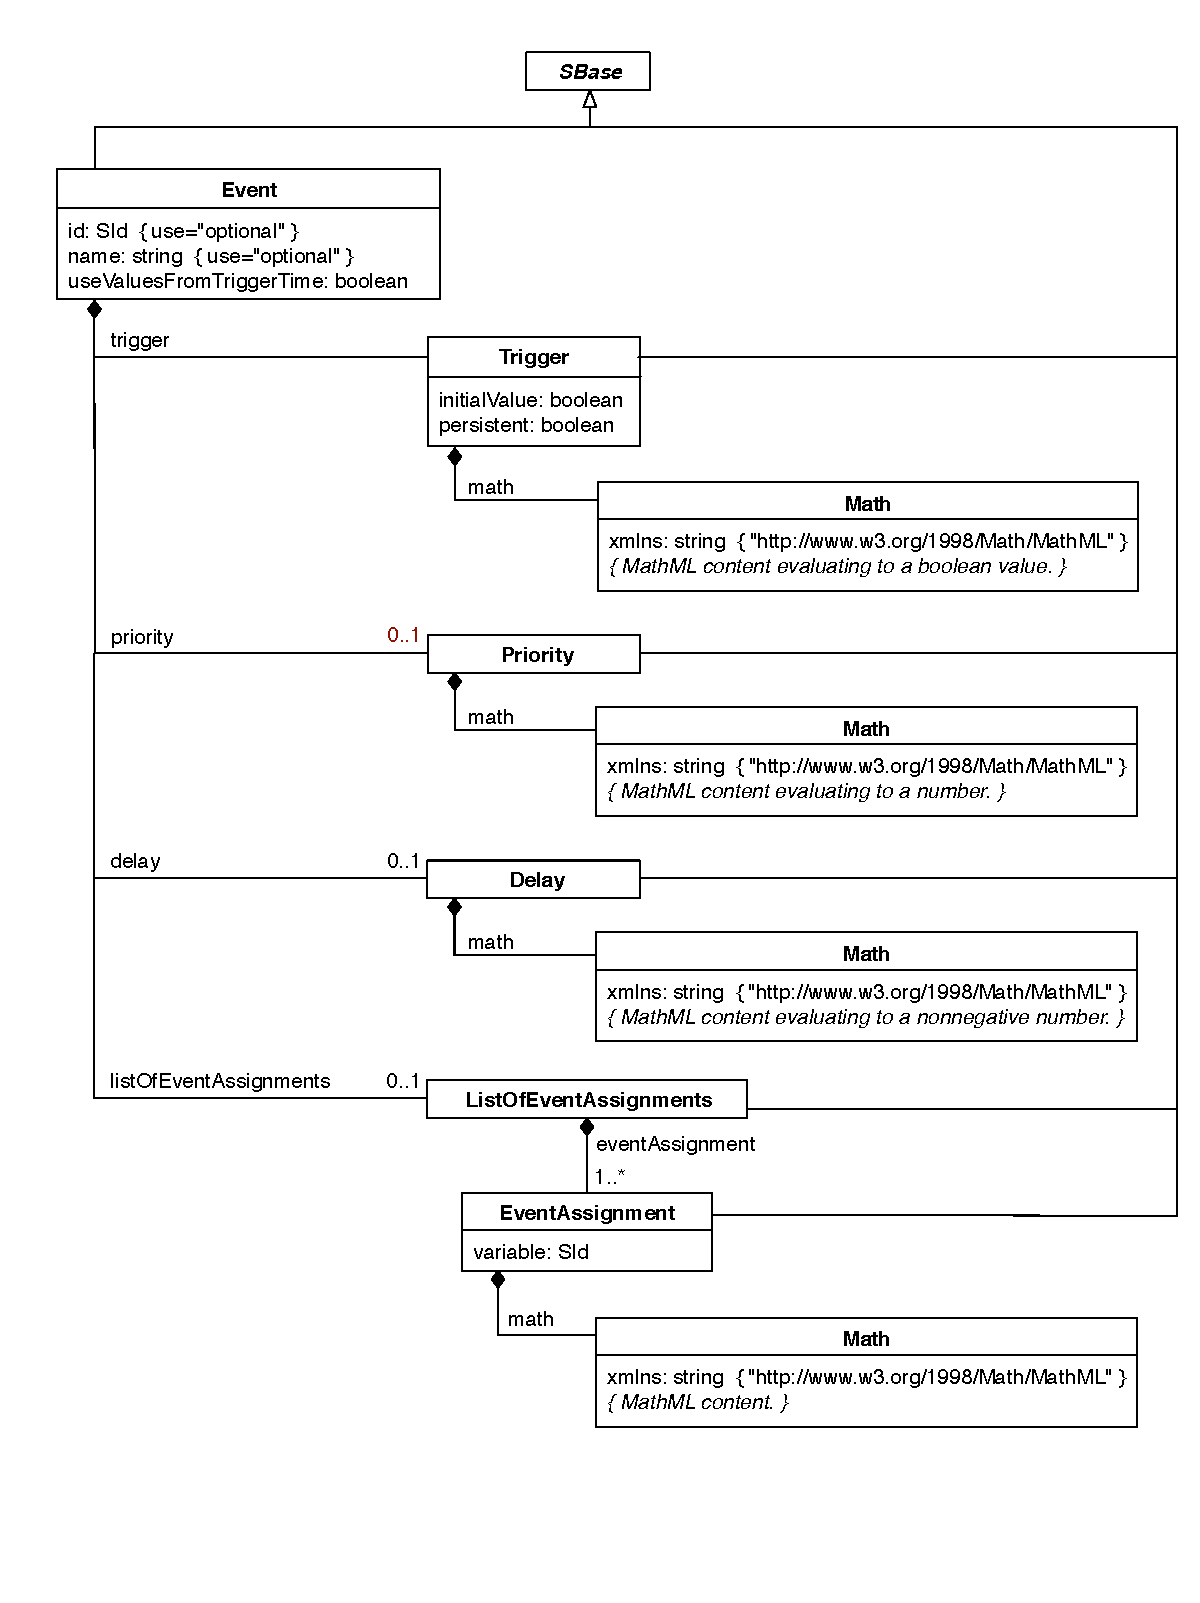
\includegraphics[scale=0.8]{figs/event-uml}
  \caption{The definitions of \Event, \Trigger, \Delay
      and \EventAssignment, and the container class
      \ListOfEventAssignments.}
  \label{fig:event}
\end{figure}


\subsubsection{\class{Event}}

An \Event definition has two required parts: a
trigger condition and at least one \EventAssignment.  In
  addition, an event can include an optional delay.  These features
  of \Event are described below.

\paragraph{The \token{id} and \token{name} attributes}
\label{sec:event-id-name}

As with most components in SBML, an \Event has \token{id} and
\token{name} attributes, but in the case of \Event, both are optional.
These attributes operate in the manner described in
Section~\ref{sec:idnameattribs}.


\paragraph{The optional \token{sboTerm} attribute on \class{Event}}
\label{sec:event-sboterm}

\Event  inherits an optional \token{sboTerm}
attribute of type \primtype{SBOTerm} from its parent
class \SBase (see Sections~\ref{sec:sboterm-type}
and~\ref{sec:sboTerm}).  When a value is given to this
attribute in a  \Event instance, it should be an
SBO identifier belonging to the branch for type  \Event
indicated in Table~\ref{tab:sboterm-availability}.  The relationship is
of the form ``the event \emph{is a} X'', where X is
the SBO term.  The term chosen should be the most precise (narrow)
one that captures the role of the event  in the model.

As discussed in Section~\ref{sec:sboTerm}, SBO labels are optional
information on a model.  Applications are free to ignore
\token{sboTerm} values.  A model must be interpretable without the
benefit of SBO labels.



\paragraph{The \token{useValuesFromTriggerTime} attribute}
\label{sec:event-usevaluesfromtriggertime}

The optional \Delay on \Event means there are two times to
consider when computing the results of an event: the time at which
the event \emph{fires}, and the time at which assignments are
\emph{executed}.  It is also possible to distinguish between the
time at which the \EventAssignment's expression is calculated, and
the time at which the assignment is made: the expression could be
evaluated at the same time the assignments are
performed, i.e., when the event is \emph{executed}, but it could
also be defined to be evaluated at the time the event
\emph{fired}.


\subsubsection{\class{Trigger}}
\label{sec:trigger}
\label{sec:event-trigger}

As shown in Figure~\ref{fig:event}, the \token{trigger} element of
an \Event must contain exactly one object of class \Trigger.  This
object contains one \token{math} element containing a MathML
expression.  The expression must evaluate to a value of type
\primtype{boolean}.  The exact moment at which the expression
evaluates to \val{true} is the time point when the \Event is
\emph{fired}.

An event only fires when its \Trigger expression makes the
transition in value from \val{false} to \val{true}.  The event
will also fire at any future time points when the \token{trigger}
make this transition; in other words, an event can fire multiple
times during a simulation if its trigger condition makes the
transition from \val{false} to \val{true} more than once.

An important question is whether an event can fire prior to, or
at, initial simulation time, \ie $t \leq 0$.  The answer is no: an
event can only be triggered immediately after initial simulation
time \ie $t > 0$.


\paragraph{The optional \token{sboTerm} attribute on \class{Trigger}}
\label{sec:trigger-sboterm}

\Trigger  inherits an optional \token{sboTerm}
attribute of type \primtype{SBOTerm} from its parent
class \SBase (see Sections~\ref{sec:sboterm-type}
and~\ref{sec:sboTerm}).  When a value is given to this
attribute in a  \Trigger instance, it should be an
SBO identifier belonging to the branch for type  \Trigger
indicated in Table~\ref{tab:sboterm-availability}.  The relationship is
of the form ``the trigger \emph{is a} X'', where X is
the SBO term.  The term chosen should be the most precise (narrow)
one that captures the role of the trigger  in the model.

As discussed in Section~\ref{sec:sboTerm}, SBO labels are optional
information on a model.  Applications are free to ignore
\token{sboTerm} values.  A model must be interpretable without the
benefit of SBO labels.

\subsubsection{\class{Delay}}
\label{sec:event-delay}

As shown in Figure~\ref{fig:event}, an \Event object can contain
an optional \token{delay} element of class \Delay.  The \Delay is
derived from \SBase and contains a mathematical formula stored in
\token{math}.  The formula is used to compute the length of time
between when the event has \emph{fired} and when the event's
assignments (see below) are actually \emph{executed}.  If no delay
is present on a given \Event, a time delay of zero is assumed.

The expression in the \Delay object's \token{math} element must be evaluated at the time the
event is \emph{fired}.  The expression must always evaluate to a
nonnegative number (otherwise, a nonsensical situation could arise
where an event is defined to fire before it is triggered!).  


\paragraph{Units of delay expressions}

The units of the numerical value computed by a \Delay instance's
\token{math} expression should match the model's units of
\quantity{time} (meaning the definition of the \val{time} units in
the model; see Section~\ref{sec:predefined-units}).  Note that, as
in other cases of MathML expressions in SBML, units are \emph{not}
predefined or assumed.  As discussed in
Section~\ref{sec:operator-arg-types}, literal numbers (\ie numbers
enclosed in MathML \token{cn} elements) or expressions containing
only literal numbers and/or \Parameter objects without declared
units, are considered to have unspecified units.  In such cases,
the correspondence between the needed units and the (unknown)
units of the \Delay \token{math} expression cannot be proven, and
while such expressions are not considered inconsistent, all that
can be assumed by model interpreters (whether software or human)
is that the units \emph{may} be consistent.

The following \Event example fragment helps illustrate this:
\label{sec:event:delay:example}

\begin{example}
<model>
    ...
    <listOfEvents>
        <event useValuesFromTriggerTime="true">
            ...
            <delay>
                <math xmlns="http://www.w3.org/1998/Math/MathML">
                    <cn> 10 </cn>
                </math>
            </delay>
            ...
        </event>
    </listOfEvents>
    ...
</model>
\end{example}

Note that the \val{<cn> 10 </cn>} within the mathematical formula has
no specified units attached to it. As Section~\ref{sec:bp:event:delay} describes 
it is \emph{best practice} to use a parameter with time units instead to clarify 
the time units. 

\paragraph{The optional \token{sboTerm} attribute on \class{Delay}}
\label{sec:delay-sboterm}

\Delay  inherits an optional \token{sboTerm}
attribute of type \primtype{SBOTerm} from its parent
class \SBase (see Sections~\ref{sec:sboterm-type}
and~\ref{sec:sboTerm}).  When a value is given to this
attribute in a  \Delay instance, it should be an
SBO identifier belonging to the branch for type  \Delay
indicated in Table~\ref{tab:sboterm-availability}.  The relationship is
of the form ``the delay \emph{is a} X'', where X is
the SBO term.  The term chosen should be the most precise (narrow)
one that captures the role of the delay  in the model.

As discussed in Section~\ref{sec:sboTerm}, SBO labels are optional
information on a model.  Applications are free to ignore
\token{sboTerm} values.  A model must be interpretable without the
benefit of SBO labels.



\subsubsection{\class{EventAssignment}}
\label{sec:eventassignment}
\label{sec:listofeventassignments}

\Event contains a mandatory element called
\token{listOfEventAssignments}, of class \ListOfEventAssignments.
In every instance of an event definition in a model, the object's
\token{listOfEventAssignments} element must have a non-empty list
of one or more \token{eventAssignment} elements of class
\EventAssignment.  The object class \EventAssignment has one
required attribute, \token{variable}, and a required element,
\token{math}.  Being derived from \SBase, it also has all the
usual attributes and elements of its parent class.

An ``event assignment'' has effect when the event is
\emph{executed}; that is, at the end of any given delay period (if
given) following the moment that the \Event is triggered.  See
Section~\ref{sec:events-semantics} below for more information
about events and event assignments in SBML.


\paragraph{The \token{variable} attribute}

The \token{variable} attribute is of type \primtype{SIdRef} and can
contain the identifier of a \Compartment, \Species, \SpeciesReference,
or \Parameter instance defined in the model.  
When the event is executed, the value of
the model component identified by \token{variable} is changed by
the \EventAssignment to the value computed by the \token{math}
element; that is, a species' quantity, species reference's stoichiometry, 
compartment's size or parameter's value are reset to the value 
computed by \token{math}.

Certain restrictions are placed on what can appear in
\token{variable}:
\begin{itemize}
  
\item The object identified by the value of the \token{variable}
  attribute must not have its \token{constant} attribute set 
  to \val{true}.  (Constants cannot be affected by events.)
  
\item The \token{variable} attribute must not contain the identifier
  of a reaction; only species, compartment and parameter values
  may be set by an \Event.
  
\item The value of every \token{variable} attribute must be unique
  among the set of \EventAssignment objects within a given
  \Event instance.  In other words, a single event cannot have
  multiple \EventAssignment{}s assigning the same variable.  (All
  of them would be performed at the same time, when that
  particular \Event triggers, resulting in indeterminacy.)
  Separate \Event instances can refer to the same variable.
  
\item A variable cannot be assigned a value in an \EventAssignment
  object instance and also be assigned a value by an
  \AssignmentRule, \ie the value of the \token{variable} attribute
  in an \EventAssignment instance cannot be the same as the value
  of a \token{variable} attribute in a \AssignmentRule instance.
  (Assignment rules hold at all times, therefore it would be
  inconsistent to also define an event that reassigns the value of
  the same variable.)

\end{itemize}



Note that the time of assignment of the object identified by the
value of \token{variable} is always the time at which the \Event
is \emph{executed}, not when it is \emph{fired}.  The timing is
controlled by the optional \Delay in an \Event.  The time of
assignment is not affected by the \token{useValuesFromTriggerTime}
attribute on \Event---that attribute affects the time at which the
\EventAssignment's \token{math} expression is evaluated.  In other
words, SBML allows decoupling the time at which the
\token{variable} is assigned from the time at which its value
expression is calculated.




\paragraph{The optional \token{sboTerm} attribute on \class{EventAssignment}}
\label{sec:eventassignment-sboterm}

\EventAssignment   inherits an optional \token{sboTerm}
attribute of type \primtype{SBOTerm} from its parent
class \SBase (see Sections~\ref{sec:sboterm-type}
and~\ref{sec:sboTerm}).  When a value is given to this
attribute in a  \EventAssignment  instance, it should be an
SBO identifier belonging to the branch for type  \EventAssignment 
indicated in Table~\ref{tab:sboterm-availability}.  The relationship is
of the form ``the event assignment \emph{is a} X'', where X is
the SBO term.  The term chosen should be the most precise (narrow)
one that captures the role of the event assignment  in the model.

As discussed in Section~\ref{sec:sboTerm}, SBO labels are optional
information on a model.  Applications are free to ignore
\token{sboTerm} values.  A model must be interpretable without the
benefit of SBO labels.


\paragraph{\class{EventAssignment}'s \token{math}}

The \token{math} element contains a MathML expression that defines
the new value of the object identified by the \token{variable}.

The time at which this expression is evaluated is determined by
\Event's \token{useValuesFromTriggerTime} attribute.  If the
attribute value is \val{true}, the expression must
be evaluated when the event is \emph{fired}; more precisely, the
values of identifiers occurring in MathML \token{ci} attributes in
the \EventAssignment's \token{math} expression are the values they
have at the point when the event \emph{fired}.  If, instead,
\token{useValuesFromTriggerTime}'s value is \val{false}, it means
the values at \emph{execution} time should be used; that is, the
values of identifiers occurring in MathML \token{ci} attributes in
the \EventAssignment's \token{math} expression are the values they
have at the point when the event \emph{executed}.


\paragraph{Units of the \token{math} formula in \class{EventAssignment}}

In all cases, as would be expected, the units of the formula
contained in the \token{math} element of
\EventAssignment should be consistent with the units of the object
identified by the \token{variable} attribute.  More
precisely:
\begin{itemize}
  
\item \emph{In the case of a species}, an \EventAssignment sets
  the referenced species' quantity (\quantity{concentration} or
  \quantity{amount of substance}) to the value determined by the
  formula in \token{math}.  The units of the \token{math} formula
  should be identical to the \emph{units of the species} as defined
  in Section~\ref{sec:species-units}.
  
\item \emph{In the case of a species reference}, an \EventAssignment sets
  the stoichiometry of the referenced \SpeciesReference to that determined by the
  formula in \token{math}. 

\item \emph{In the case of a compartment}, an \EventAssignment
  sets the referenced compartment's size to the size determined by
  the formula in \token{math}.  The overall units of the formula
  should be identical to the units specified for the size of the
  compartment identified by the value of the \EventAssignment's
  \token{variable} attribute.  (See
  Section~\ref{sec:compartment-units} for an explanation of how
  the units of the compartment's size are determined.)
  
\item \emph{In the case of a parameter}, an \EventAssignment sets
  the referenced parameter's value to that determined by the
  formula in \token{math}.  The overall units of the formula should
  be identical to the units defined for the parameter identified
  by the value of the \EventAssignment's \token{variable}
  attribute.  (See Section~\ref{sec:parameter-units} for
  an explanation of how the units of the parameter are
  determined.)

\end{itemize}



Note that the formula placed in the \token{math} element
has no assumed units.  The consistency of the units of the
formula, and the units of the entity which the assignment affects,
should be explicitly established just as in the case of the value of
\token{delay}.


% FIXME explain how to handle species quantities if an event sets
% both a species and a compartment size at the same time.



\subsubsection{Example \class{Event} definitions}

A example of an \Event object follows.  This structure makes the
assignment $k_2 = 0$ at the point when $P_1 \leq P_2$:

\begin{example}

<event>
    ...
    <listOfUnitDefinitions>
        <unitDefinition id="per_second">
            <listOfUnits>
                <unit kind="second" exponent="-1" multiplier="1" scale="0"/>
            </listOfUnits>
        </unitDefinition>
    </listOfUnitDefinitions>
    ...
    <listOfParameters>
        ...
        <parameter id="k2" value="0.05" units="per_second" constant="false"/>
        <parameter id="k2reset" value="0.0" units="per_second" constant="true"/>
        ...
    </listOfParameters>
    ...
    <listOfEvents>
        <event useValuesfromTriggerTime="true">
            <trigger>
                <math xmlns="http://www.w3.org/1998/Math/MathML">
                    <apply>
                        <leq/>
                        <ci> P_1 </ci>
                        <ci> P_2 </ci>
                    </apply>
                </math>
            </trigger>
            <listOfEventAssignments>
                <eventAssignment variable="k2">
                    <math xmlns="http://www.w3.org/1998/Math/MathML">
                        <ci> k2reset </ci>
                    </math>
                </eventAssignment>
            <listOfEventAssignments>
        </event>
    </listOfEvents>
    ...
</model>

\end{example}

A complete example of a model using events is given in
Section~\ref{sec:eventeg}.


\subsubsection{Detailed semantics of events}
\label{sec:events-semantics}

The description of events above describes the action of events in
isolation from each other.  This section describes how events
interact.

Events whose \token{trigger} expression is true at the start of a
simulation do not \emph{fire} at the start of the simulation ($t =
0$).  Events \emph{fire} only when the trigger \emph{becomes}
true, \ie the trigger expression transitions from false to true,
which cannot happen at $t = 0$ but can happen at $t > 0$.

Any transition of a \token{trigger} expression from \val{false} to
\val{true} will cause an \token{event} to \emph{fire}.  Consider
an \token{event} $E$ with delay $d$ where the \token{trigger}
expression makes a transition from false to true at times $t_1$
and $t_2$.  The \EventAssignment object will have effect at
$t_1+d$ and $t_2+d$ irrespective of the relative times of $t_1$
and $t_2$. For example events can ``overlap'' so that $t_1 < t_2 <
t_1+d$ still causes an event assignments to occur at $t_1+d$ and
$t_2+d$.

It is possible for events to \emph{fire} other events, \ie an
event assignment can cause an event to \emph{fire}, therefore it
is possible for a model to be entirely encoded in \Event
objects.

It is entirely possible for two events to be \emph{executed}
simultaneously in simulated time.  It is assumed that, although
the precise time at which these events are \emph{executed} is not
resolved beyond the given point in simulated time, the order in
which the events occur is resolved.  This order can be significant
in determining the overall outcome of a given simulation. SBML
Level 2 does not define the algorithm for determining this order
(the tie-breaking algorithm).  As a result, the outcomes of
simulations involving events may vary when simultaneous events
occur during simulation.  It is anticipated that future versions
or levels of SBML will define a specific set of tie-breaking
algorithms and a mechanism for models to indicate which algorithm
should be applied during simulation.

Despite the absence of a specific tie-breaking algorithm, SBML
event simulation is constrained as follows. When an event $X$
\emph{fires} another event $Y$ and event $Y$ has zero delay then
event $Y$ is added to the existing set of simultaneous events that
are pending \emph{execution}.  Events such as $Y$ do not have a
special priority or ordering within the tie-breaking algorithm.
Events $X$ and $Y$ form a cascade of events at the same point in
simulation time.  All events in a model are open to being in a
cascade.  The position of an event in the event list does not
affect whether it can be in the cascade: $Y$ can be triggered
whether it is before or after $X$ in the list of events.  A
cascade of events can be infinite (never terminate).  When this
occurs a simulator should indicate this has occurred; \ie it is
incorrect for the simulator to arbitrarily break the cascade and
continue the simulation without at least indicating the infinite
cascade occurred. A variable can change more than once when
processing simultaneous events at simulation time $t$.  The model
behavior (output) for such a variable is the value of the variable
at the end of processing all the simultaneous events at time $t$.











% -----------------------------------------------------------------------------
% chunks of text that maybe will be useful some day:
% -----------------------------------------------------------------------------

% Here it pays to reflect more carefully about what a reaction is.
% A reaction represents a process occuring over time.  the process
% acts on the reactants, transforming them in some way into the
% products.  the transformation may be anything from a change in
% the nature of the reactants to a simple relocation without any
% change to the nature of the reactants; for the purpose of talking
% about the speed of the reaction it does not matter.

% The ``kinetic law'' is a statement about the speed at which the
% process takes place, or more precisely, the frequency of the
% events occuring in this process.  It is by default in terms of
% moles per second, which has some intuitive appeal when dealing
% with chemical substances.  But notice that a ``mole'' is actually
% a statement about numbers of ``things'': it is 6.02e23 of whatever
% is involved.  In the case of chemical species, it is molecules of
% the substance.  To say ``one mole of'' is a shorthand way of
% saying ``6.02e23 molecules of''.  Thus, a reaction expressed as
% ``X moles per second'' is a statement that the process involves
% ``(X times 6.02e23) items per second''.

% 1 kg/sec is 1 kg/sec

% If in a reaction, the units of the species are the same as the
% reaction's substance units (default mole, redefinable by
% redefining ``substance''; sec section x), then the stoichiometries
% represent simply the ratios of the participating species: 1 mole
% of this to 2 moles of that, and so on.  If instead the species are
% given in different units, then the species quantities must be
% converted to be consistent with the units of the reaction.  Thus,
% the SBML stoichiometry may then have to incorporate a conversion:
% the stoichiometry will represent the product of the biochemical
% reaction stoichiometry and a ratio between the species substance
% and the reaction substance.

% don't forget units of reaction id


% ---

% started trying to generate the event diagram in pgf but
% it's too hard.

%   \begin{tikzpicture}[level distance=2in]
%     \node[left=1.15in,above=0.35in] (a) { \emptyClassbox{\textsl{SBase}} };
%     \node[left=0.75in] (b) {
%       \begin{classbox}{Event}
%         id: SId  \{ use="optional" \}     \\
%         name: string \{ use="optional" \} \\
%       \end{classbox} 
%     }
%     [diamond-,edge from parent fork right,grow=right,sibling distance=0.6in]
%     child {node[right=0.15in] (c) { \emptyClassbox{ListOfEventAssignments} }
%       child {node (f) {
%           \begin{classbox}{EventAssignment}
%             variable: SIdRef                                                   \\
%           \end{classbox}
%         }}
%       child {node (g) {
%           \begin{classbox}{Math}
%             xmlns: string \{ "http://www.w3.org/1998/Math/MathML" \} \\
%             \{ \emph{\mathml content} \} \\
%           \end{classbox}
%         }}
%     }
%     child {node[right=0.15in] (d) { \emptyClassbox{Delay} }
%     }
%     child {node[right=0.15in] (d) { \emptyClassbox{Trigger} }
%     }
      
% junk

%      [diamond-,edge from parent fork down,sibling distance=0.6in]
%         \begin{classbox}{Delay}
%           xmlns: string \{ "http://www.w3.org/1998/Math/MathML" \} \\
%           \{ \emph{\mathml content} \} \\
%         \end{classbox}
%       }}
%     child {node[right=0.15in] (e) {
%         \begin{classbox}{Trigger}
%           xmlns: string \{ "http://www.w3.org/1998/Math/MathML" \} \\
%           \{ \emph{\mathml content evaluating to a boolean value} \} \\
%         \end{classbox}
%       }}
%    ;
%           \begin{classbox}{EventAssignment}
%             variable: SIdRef                                                   \\
%             math: Math \{ namespace="http://www.w3.org/1998/Math/MathML" \} \\
%           \end{classbox}
%      \draw[open triangle 60-] (a) -- (b);
%      \draw node[left=0.4in,above=0.375in] {\textsf{math}};
%      \draw node[left=0.3in,below=0.225in] {\textsf{message}};
%      \draw node[left=-0.15in,below=0.215in] {\textsf{0..1}};
%  \end{tikzpicture}

%   
%   \vspace*{2ex}
%   \begin{classbox}{Trigger}
%     math: Math \{ namespace="http://www.w3.org/1998/Math/MathML" \} \\
%   \end{classbox}
%   \vspace*{2ex}
%   \begin{classbox}{Delay}
%     math: Math \{ namespace="http://www.w3.org/1998/Math/MathML" \} \\
%   \end{classbox}
%   \vspace*{2ex}
%   
